%!TEX root = ../thesis.tex

\thispagestyle{myheadings}

\graphicspath{{Body/Figures/ExperimentalOverview/Decay/}{Body/Figures/TrackingFigures/TrackerPics/}{Body/Figures/ExperimentalOverview/Ring/}{Body/Figures/ExperimentalOverview/Accelerator/}{Body/Figures/ExperimentalOverview/Beam/}{Body/Figures/ExperimentalOverview/Auxiliary/}{Body/Figures/MagneticField/}}

\chapter{Principal Techniques of E989}
\label{chapter:E989}

A particle with non-zero spin in a magnetic field will experience a torque which attempts to line up the magnetic dipole moment of the particle with the external field. Because of this, in a dipole field a particle's spin will turn at the spin precession frequency \cite{Jackson}
        \begin{align} \label{eq:ws}
            \vec{\omega}_{s} = -g\frac{q}{2m}\vec{B} - (1-\gamma)\frac{q}{\gamma m}\vec{B},
        \end{align}
where $m$ is the particle's mass, $q = \pm e$ where $e$ is the positive elementary charge, \g is the g-factor, $\gamma$ is the Lorentz relativistic factor, and $B$ is an external magnetic field. The first term is the usual Larmor frequency and the second term is a relativistic correction to the precession frequency in an accelerating frame called Thomas precession. Similarly, a particle with some momentum perpendicular to the magnetic field will orbit at the cyclotron frequency
        \begin{align} \label{eq:wc}
            \vec{\omega}_{c} = -\frac{q}{\gamma m}\vec{B}.
        \end{align}
By taking the difference between these two frequencies we arrive at the ``spin difference frequency''
        \begin{align} \label{eq:wasimple}
            \vec{\omega}_{a} = \vec{\omega}_{s} - \vec{\omega}_{c} = -\frac{g-2}{2}\frac{q}{m}\vec{B} = - a \frac{q}{m}\vec{B},
        \end{align}
a frequency that is directly proportional to the anomaly $a$. If $g = 2$, as in a Dirac theory, then the particle's spin would turn at the same rate as the momentum vector, and \wa would be identically zero. If \wa for a muon and the external magnetic dipole field can be measured, then the anomalous magnetic moment of the muon \amu can be determined.

As will be detailed in \secref{sec:MagneticField}, the measurement of the magnetic field is related to the Larmor precession frequency of free protons in water 
        \begin{align} \label{eq:wp}
            \omega_{p} = -g_{p} \frac{e}{2m_{p}} B,
        \end{align}
where $g_{p}$ and $m_{p}$ are the g-factor and mass of the proton respectively. Replacing $B$ and solving for \amu, we arrive at 
        \begin{align} \label{eq:amu}
            a_{\mu} = \frac{g_{p}}{2} \frac{\omega_{a}}{\omega_{p}} \frac{m_{\mu}}{m_{p}}.
        \end{align}
Using the magnetic moment formulae for the proton, electron, and muon as shown in \equref{eq:magneticmoment}, \equref{eq:amu} can be transformed into
        \begin{align} 
            a_{\mu} &= \frac{g_{e}}{2} \frac{\omega_{a}}{\omega_{p}} \frac{m_{\mu}}{m_{e}} \frac{\mu_{p}}{\mu_{e}}, \label{eq:amuratios}
        \end{align}
where the $p$, $e$, and $\mu$ subscripts stand for the relevant quantities for the proton, electron, and muon respectively. The experimental error on \amu then becomes the quadrature sum of each individual quantity error. As mentioned in \secref{sec:BSM} the electron g-factor $g_{e}$ has been measured to extremely high precision, $\SI{0.26}{ppt}$ \cite{CODATA,ElectronMDM}. The muon-electron mass ratio, $m_{\mu}/m_{e}$, has been measured to \SI{22}{ppb} \cite{CODATA,MuoniumHyperfine}. Finally the proton-electron magnetic moment ratio, $\mu_{p}/\mu_{e}$, has been measured to \SI{3}{ppb} \cite{CODATA}. These are small compared to the target statistical error on \wa of $\SI{100}{ppb}$, and target systematic errors on \wa and $\omega_{p}$, both at $\SI{70}{ppb}$\footnote{The measurement of $\omega_{p}$ has negligible statistical error.}. These errors added in quadrature is approximately $\SI{140}{ppb}$, which is the target of the E989 experiment.



% Using the magnetic moment formulae for the proton, electron, and muon as shown in \equref{eq:magneticmoment}, \equref{eq:amu} can be transformed to either of the following consistent equations:
%         \begin{align} 
%             a_{\mu} &= \frac{g_{e}}{2} \frac{\omega_{a}}{\omega_{p}} \frac{m_{\mu}}{m_{e}} \frac{\mu_{p}}{\mu_{e}} \label{eq:amuratios} \\ 
%             a_{\mu} &= \frac{\omega_{a}/\omega_{p}}{\lambda - \omega_{a}/\omega_{p}} \label{eq:amulambda}
%         \end{align}
% Here the $p$, $e$, and $\mu$ subscripts stand for the relevant quantities for the proton, electron, and muon respectively. In the second equation $\lambda = \mu_{\mu}/\mu_{p}$. As mentioned before the electron g-factor $g_{e}$ has been measured to extremely high precision, 0.26 ppt \cite{ElectronMDM,CODATA}. The muon-electron mass ratio $m_{\mu}/m_{e}$ and muon-proton magnetic moment ratio $\lambda$ have been measured to 22 ppb \cite{CODATA,MuoniumHyperfine}. Finally the proton-electron magnetic moment ratio $\mu_{p}/\mu_{e}$ has been measured to 3 ppb \cite{CODATA}. The errors on these terms are small compared to the target uncertainty for E989 of 140 ppb, the measurement of which now comes down to measuring the ratio $\omega_{a}/\omega_{p}$. 






\section{Measuring \texorpdfstring{\wa}{wa}}
\label{section:WaIntro}

How can \wa for muons be measured? The answer lies with two key points in the dynamics of muon decay. Positive muons decay to a positron and two neutrinos, as shown in \figref{fig:mudecay}. The first point is that because of the parity violating nature of the weak interaction, the decay positron will be preferentially emitted right-handed, with its spin directed in the same direction as its momentum \cite{Bucksbaum}. The second key point is that angular momentum must be conserved. Consider the most extreme examples of maximum and minimum energy positrons as shown in \figref{fig:MuonDecayImproved}. In the muon rest frame, decay positrons with maximum energy will be emitted opposite to the two neutrinos, both emitted in the same direction. Since neutrinos and anti-neutrinos must be left and right-handed respectively, thus having their spins anti-parallel and parallel to their momentum, by the law of conservation of angular momentum the positron must have its spin be parallel to the spin of the muon at the time of the decay. By the opposite argument, decay positrons emitted with minimum energy such that the neutrinos are ejected opposite to one another must have their spins be anti-parallel to that of the muon at the time of decay. Together, these two points mean that higher energy decay positrons will preferentially be emitted in directions parallel to the muon spin at the time of decay, while lower energy decay positrons will preferentially be emitted in directions anti-parallel to the muon spin at the time of the decay. 

\begin{figure}
\centering
        \begin{tikzpicture}[baseline=(o.base)]
        \begin{feynhand}
        \large
        \setlength{\feynhandlinesize}{1pt}
        \vertex [dot] (o) at (0,0);
        \vertex (a) at (-2,0) {$\mu^{+}$}; 
        \vertex (b) at (1.5,1.5) {$\overline \nu_{\mu}$}; 
        \vertex (c) at (1.5,-1.5);
        \vertex (d) at (3,0) {$\nu_{e}$};
        \vertex (e) at (3,-3) {$e^{+}$};
        \propag [anti fermion] (a) to (o);
        \propag [fermion] (b) to (o);
        \propag [boson] (o) to [edge label' = $W^{+}$] (c);
        \propag [fermion] (c) to (d);
        \propag [anti fermion] (c) to (e);
        \end{feynhand}
        \end{tikzpicture} 
\caption[Diagram for muon decay]{Diagram for muon decay. $\mu^{+}$ decay through a $W^{+}$ boson to a positron, muon anti-neutrino, and an electron neutrino. This process consists of nearly 100\% of the muon decay branching ratio, with other decay states including radiative processes.}
\label{fig:mudecay}
\end{figure}

    % \hspace{10mm}
    % \subcaptionbox{$\pi^{+}$ decay through a $W^{+}$ boson to a $\mu^{+}$.
    % \label{fig:pidecay}}
    % {
    % \centering
    %     \begin{tikzpicture}[baseline=(o.base)]
    %     \begin{feynhand}
    %     \large
    %     \setlength{\feynhandlinesize}{1pt}
    %     \vertex [dot] (o) at (0,0);
    %     \vertex (a) at (-1.5,1.5) {$u$}; 
    %     \vertex (b) at (-1.5,-1.5) {$\overline d$}; 
    %     \vertex (c) at (2,0);
    %     \vertex (d) at (3.5,1.5) {$\mu^{+}$};
    %     \vertex (e) at (3.5,-1.5) {$\nu_{\mu}$};
    %     \propag [fermion] (a) to (o);
    %     \propag [anti fermion] (b) to (o);
    %     \propag [boson] (o) to [edge label = $W^{+}$] (c);
    %     \propag [anti fermion] (c) to (d);
    %     \propag [fermion] (c) to (e);
    %     \end{feynhand}
    %     \end{tikzpicture}  
    % }


\begin{figure}
    \centering
    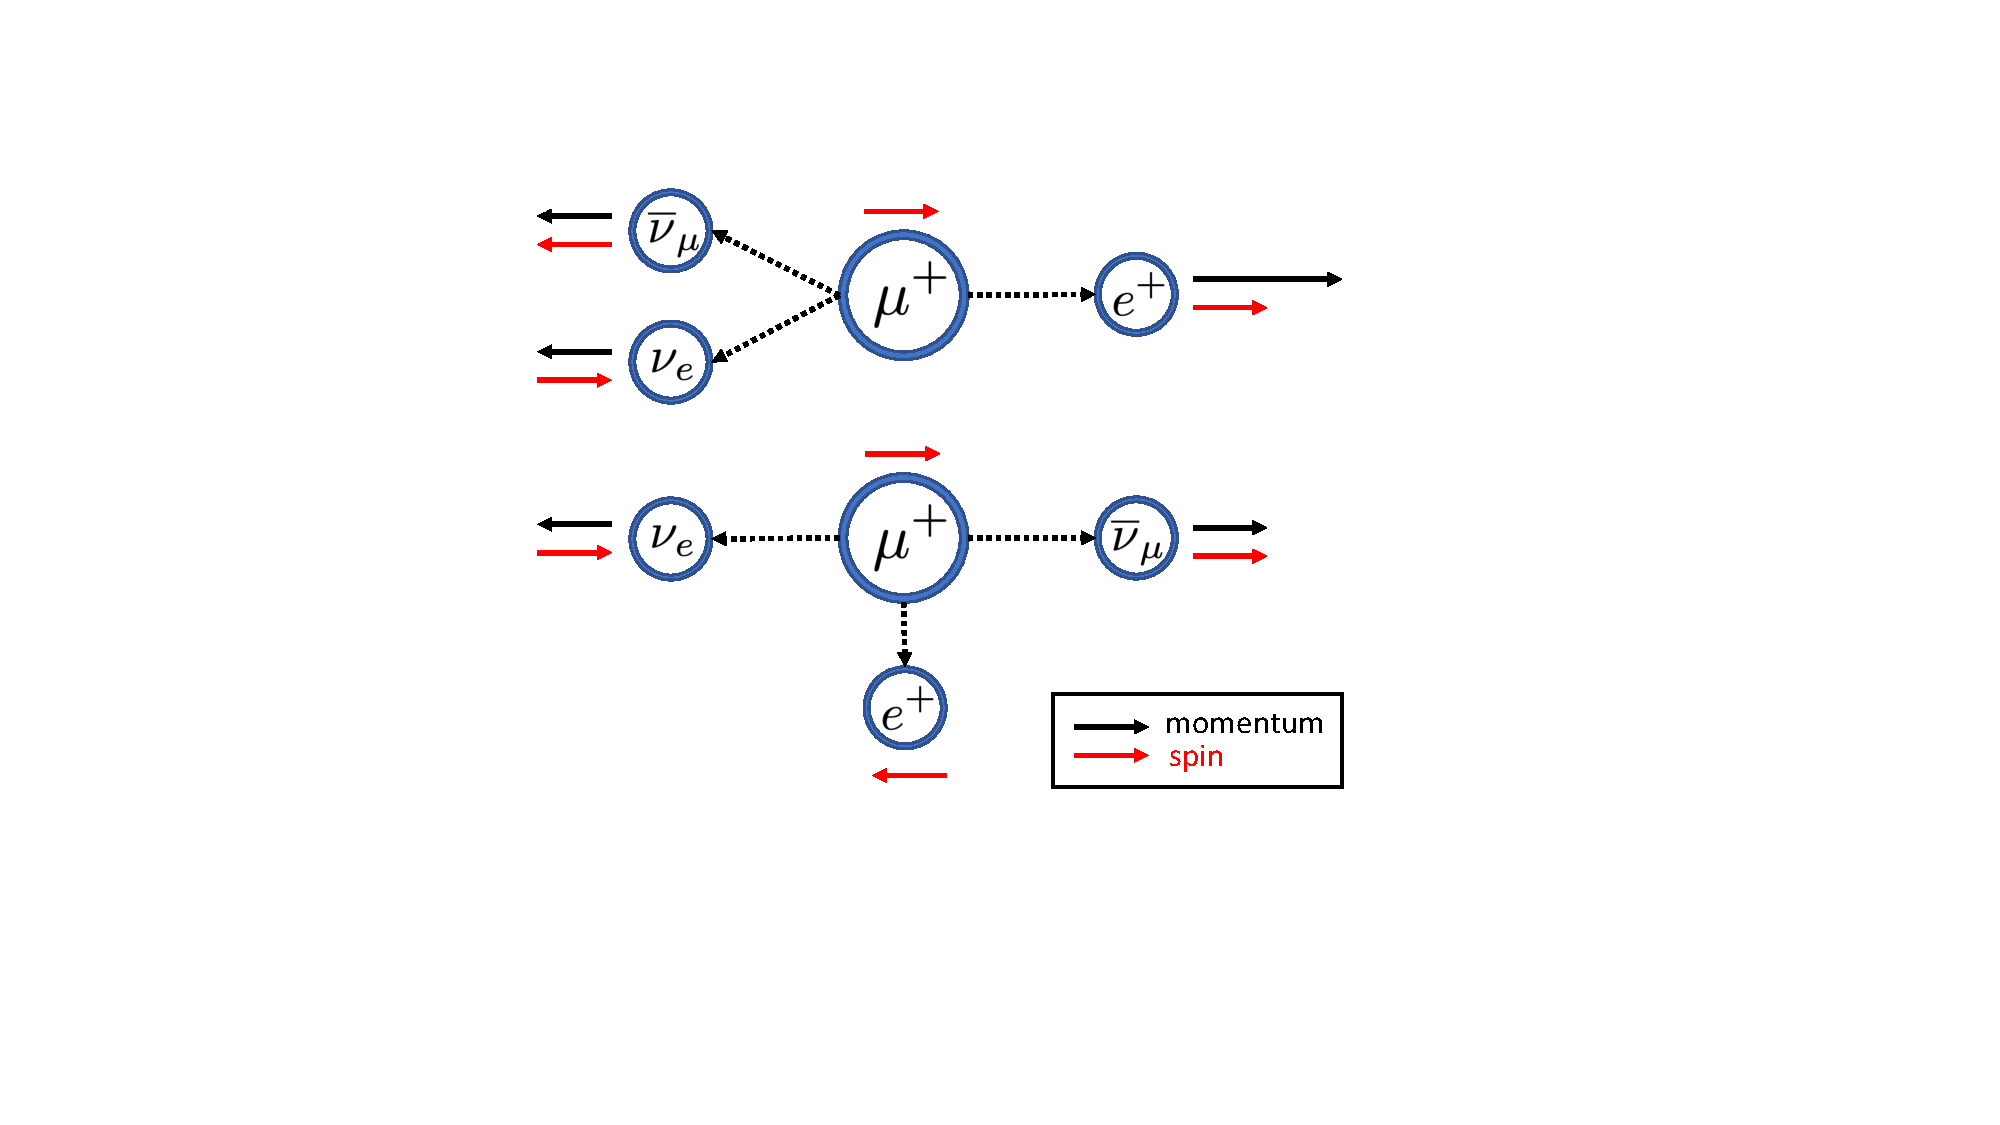
\includegraphics[width=0.6\textwidth]{MuonDecayImproved}
    \caption[Muon decay for maximum and minimum energy decay positrons]{Muon decay in the rest frame for maximum (top) and minimum (bottom) energy decay positrons. Due to the conservation of angular momentum and the single possible helicity states of the decay neutrinos, the spin of the decay positron is exactly parallel to the spin of the muon at the time of the decay for maximum energy decay positrons, or anti-parallel for minimum energy decay positrons.}
    \label{fig:MuonDecayImproved}
\end{figure}


This correlation between the direction of an emitted high energy decay positron and the spin of the muon is the signature needed to measure \wa. Muons placed within a magnetic storage ring will orbit at the cyclotron frequency and their spins will precess at the spin precession frequency. As they go around the ring they will decay to positrons whose energy and decay directions contain information about the spin of the muon. If the muon ensemble is un-polarized, then the decay distribution for all positrons will be isotropic and in general un-useful. If the muon ensemble is polarized, then the decay distribution for each muon will be the same, and allow for a measurement of \wa, as described in the following text.


The differential decay distribution for positive muons in the muon rest frame is described by \cite{Bucksbaum}
        \begin{align} \label{eq:diffdecaydist}
            dP(y, \theta) \propto N(y)[1 + A(y)\cos(\theta)]dy d\Omega,
        \end{align}
where $y=E/E_{max}$ is the energy fraction of the positron and $\theta$ is the angle between the spin of the muon and the momentum of the positron at the time of decay. $N(y)$ is the number distribution of decay positrons and $A(y)$ is the so called `asymmetry,' encoding the energy-dependent correlation between the muon spin and the decay positron direction. Here the energy of the positron is assumed to be much greater than its mass. The number distribution and asymmetry are given by \cite{Bucksbaum}
        \begin{align}
            N(y) &= 2y^{2}(3-2y), \label{eq:Nmrf} \\
            A(y) &= \frac{2y-1}{3-2y}, \label{eq:Amrf}
        \end{align}
and are shown in \figref{fig:NA2mrf}. 

\begin{figure}
\centering
    \begin{subfigure}[]{0.45\textwidth}
        \centering
        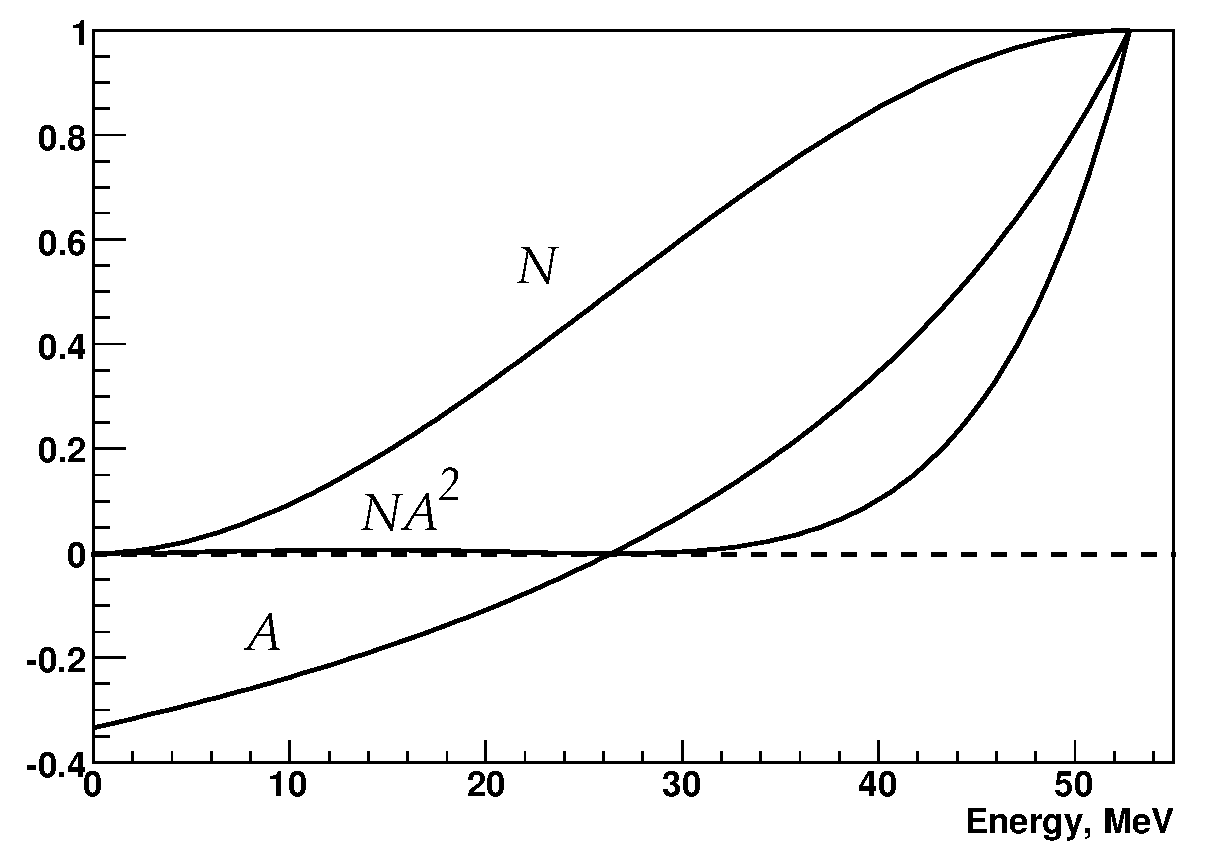
\includegraphics[width=\textwidth]{NA_mrf}
        \caption{Muon rest frame}
    \label{fig:NA2mrf}
    \end{subfigure}%
    \hspace{1cm}
    \begin{subfigure}[]{0.45\textwidth}
        \centering
        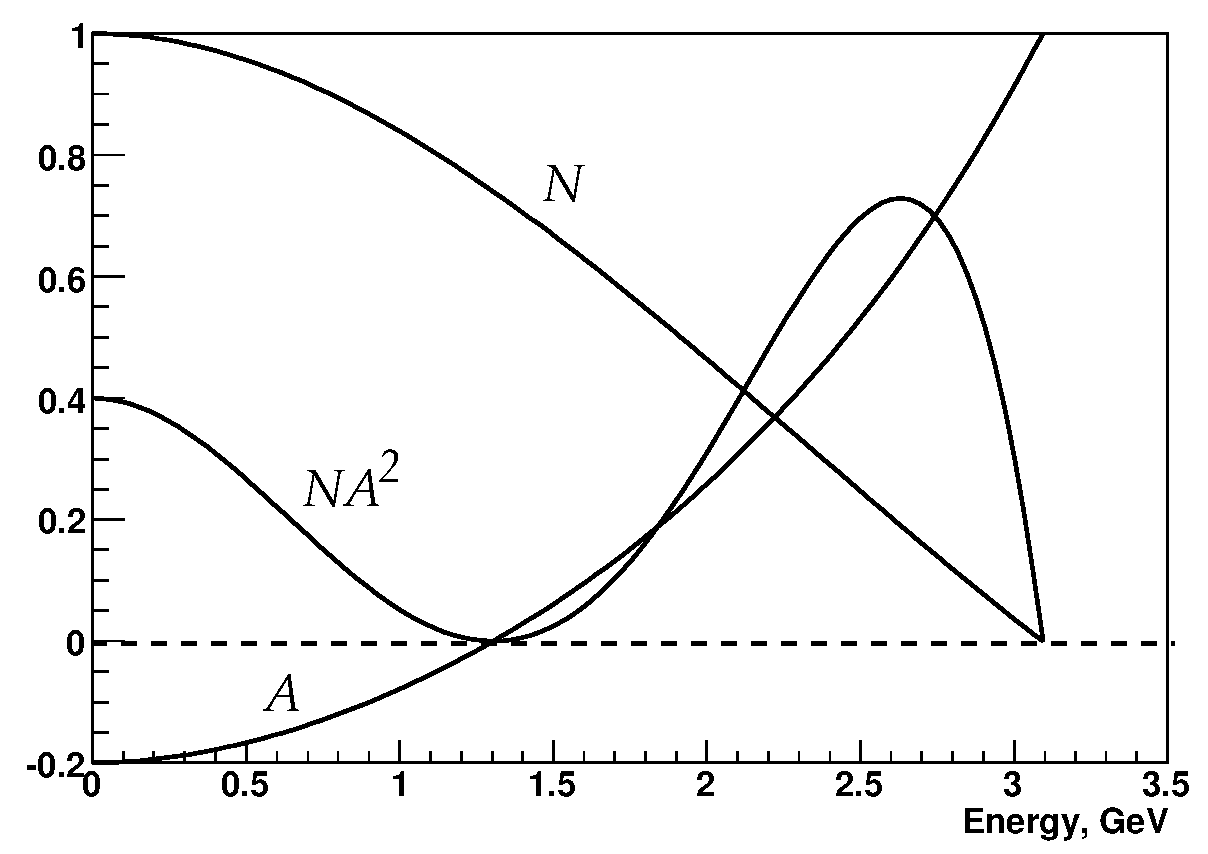
\includegraphics[width=\textwidth]{NA_lab}
        \caption{Lab frame}
    \label{fig:NA2lab}    
    \end{subfigure}
\caption[Number distribution and asymmetry for muon decay in the muon rest frame and lab frame]{Decay number distribution $N$ and asymmetry $A$ in the muon rest frame (left) and in the lab frame (right) as a function of positron energy with a maximum positron energy of 3.1 \GeV. $N$ is multiplied by arbitrary factors in both pictures.}
\label{fig:NA2}
\end{figure}

In the lab frame, nearly all high energy positrons are emitted parallel to the muon momentum, making it challenging to select purely on the decay angle of the positron. That is not a problem however, as we already know that decay positrons with the highest rest-frame energies will be emitted parallel to the muon spin at the time of decay. Essentially, the energy distribution of detected high energy positrons is modulated by \wa, or $\theta = \omega_{a}t + \phi$. The number of detected positrons at some time and energy in the lab frame for some initial number $N_{0}$ of muons can then be described by
        \begin{align}
            N_{d}(t, E) = N_{0}(E) \cdot e^{-t/\gamma\tau_{\mu}} \cdot [1 + A(E) \cos(\omega_{a}t+\phi(E))],
        \end{align}
where the $d$ subscript stands for `detected,' the muons are decaying with a lifetime of $\gamma\tau_{\mu}$, and all the relevant parameters are energy dependent. Here $N_{0}(E)$ and $A(E)$ have been transformed from Equations~\ref{eq:Nmrf} and \ref{eq:Amrf} to the lab frame:
        \begin{align}
            N_{0}(E) &\propto (y-1)(4y^{2}-5y-5), \label{eq:Nlab} \\
            A(E) &= \frac{-8y^{2}+y+1}{4y^{2}-5y-5}, \label{eq:Alab}
        \end{align}
where as a reminder $y=E/E_{max}$. Here the polarization of the muons is assumed to be unity. These relations are shown in \figref{fig:NA2lab}. All positrons above some energy threshold cut $E_{th}$ can be taken as the observable,
        \begin{align} \label{eq:5parfunc}
            N_{d}(t, E_{th}) = N_{0}(E_{th}) \cdot e^{-t/\gamma\tau_{\mu}} \cdot [1 + A(E_{th}) \cos(\omega_{a}t+\phi(E_{th}))],
        \end{align}
where the number and asymmetry of the detected positrons is now calculated by simply integrating Equations~\ref{eq:Nlab} and \ref{eq:Alab} from $y_{th}$ to 1,
        \begin{align}
            N_{0}(E_{th}) &\propto (y_{th}-1)^{2}(-y_{th}^{2}+y_{th}+3), \label{eq:Nth} \\
            A(E_{th}) &= \frac{y_{th}(2y_{th}+1)}{-y_{th}^{2}+y_{th}+3}, \label{eq:Ath}
        \end{align}
where $y_{th}=E_{th}/E_{max}$. By counting decay positrons above some energy threshold and fitting the resulting time spectrum with \equref{eq:5parfunc}, \wa can be extracted. A sample of data adhering to such a time spectrum is shown in \figref{fig:gm2wiggle}.


\begin{figure}
    \centering
    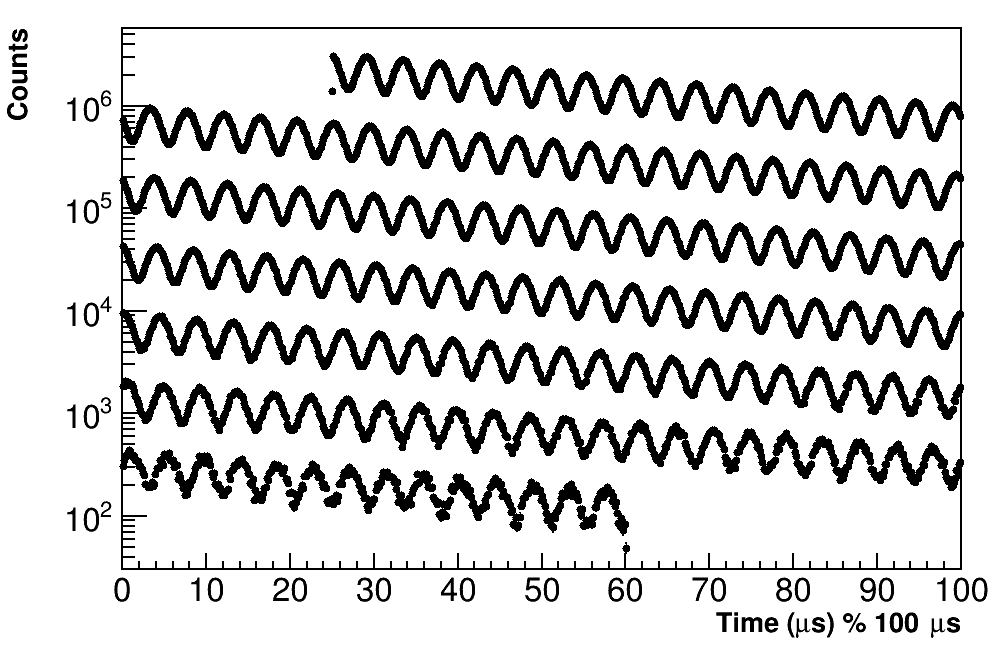
\includegraphics[width=0.9\textwidth]{gm2wiggle}
    \caption[\gmtwo time spectrum example]{The number of detected positrons above some energy threshold ($y \sim 0.55$) as a function of time, where the data plotted come from Run 1 and correspond to nearly $\SI{1e9}{}$ counts. The time axis is wrapped around every \mus{100}. See \chapref{chapter:wa} for the fitting of such a histogram.}
    \label{fig:gm2wiggle}
\end{figure}


The statistical error on the \wa measurement, assuming bin errors are Gaussian and a \chisq minimization is used with the fit function described in \equref{eq:5parfunc}, is \cite{statisticspaper}
        \begin{align} \label{eq:waprecision}
            \frac{\sigma_{\omega_{a}}}{\omega_{a}} = \frac{\sqrt{2}}{\sqrt{N_{\text{total}}}A\gamma\tau_{\mu}\omega_{a}},
        \end{align}
where $N_{\text{total}}$ is the total number of counts included in the above-threshold time spectrum. This equation assumes a weighting of one for every count included in the fitted time spectrum. Other weighting schemes exist which slightly improve the statistical precision of the \wa measurement \cite{statisticspaper}, but they are not used in this analysis. What \equref{eq:waprecision} reveals is that the statistical precision of \wa is maximized when the quantity $NA^{2}$ is at a maximum. It was found for E989 that the optimal energy threshold was about $\SI{1.7}{\GeV}$ as shown in \figref{fig:OptimalEnergyThreshold}, which includes detector acceptance effects and corresponds to an asymmetry of about $A = 0.37$. \equref{eq:waprecision} can be rearranged in order to solve for the number of positrons needed to be collected above threshold for a specific precision goal. For a statistical error of $\SI{100}{ppb}$ on \wa, the required number of positrons above threshold is approximately $\SI{170e9}{}$, determined from the values $A = 0.37$, $\gamma = 29.3$ (described later), $\tau_{\mu} = \SI{2.2}{\micro s}$, and $\omega_{a} = \SI{1.44}{\text{rad}/\micro s}$. This statistical error of \wa combined with the systematic uncertainties given in \tabref{tab:wauncertainties}, provide the total error on \wa.



\section{Measuring the magnetic field}
\label{sec:MagneticField}


In order to measure the magnetic moment of the muon to 140 ppb, the field needs to be both highly uniform, and measured to extreme precision. The E989 goal for the field measurement is 70 ppb. As shown in \equref{eq:amuratios}, the measurement of the magnetic field has equal weight to that of the precession frequency. A cross-section of the magnetic storage ring used in E989 is shown in \figref{fig:MagnetCrossSection}. It is an approximately $\SI{14}{m}$ diameter C magnet, where the muons are stored within a $\SI{4.5}{cm}$ radius cylindrical storage region at the center of a $\SI{1.451}{T}$ magnetic field. This corresponds to an approximately $\SI{0.28}{m^{3}}$ or $\SI{10}{ft^{3}}$ total volume around the inside of the ring. The magnetic field is made uniform by manipulating many magnetic `knobs' built into the \gmtwo storage ring, including the main magnet current, pole pieces, wedges, top hats, and thousands of small magnetic shims placed around the storage region, as shown in \figref{fig:MagnetCrossSection}. There is also an active feedback system which stabilizes the average magnetic field over time using current carrying coils near the storage region. After a several month shimming campaign by many members of the field team, a precision on the magnetic field of approximately $\SI{25}{ppm}$ RMS (root mean square) was achieved.

\begin{figure}
    \centering
    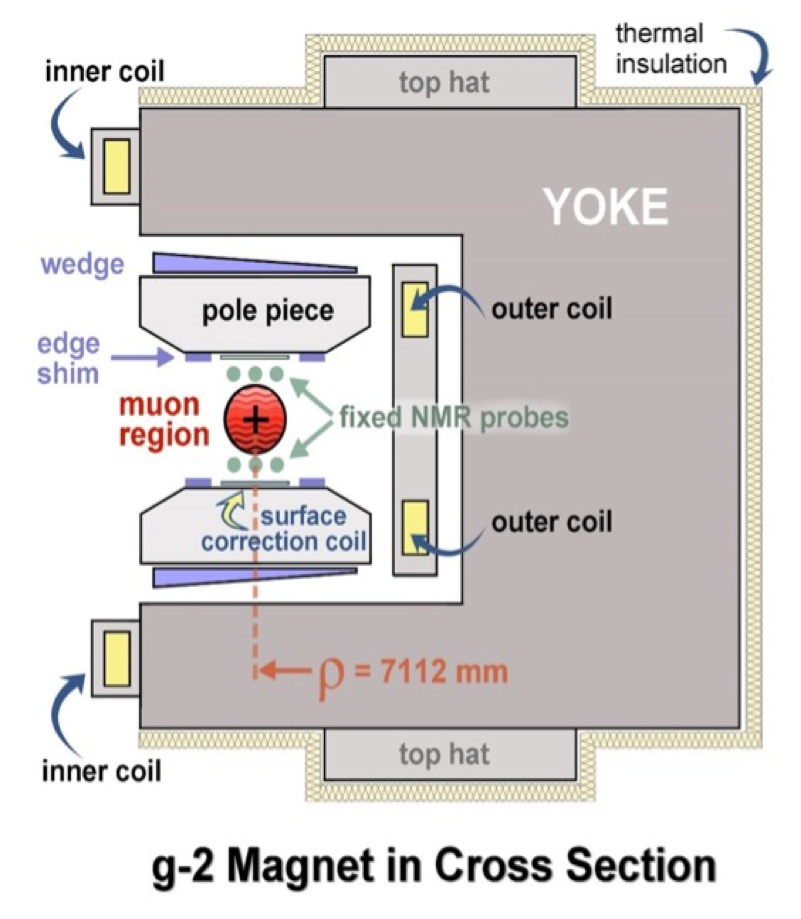
\includegraphics[width=0.6\textwidth]{MagnetCrossSection}
    \caption[Magnet cross section]{Cross-section of the \gmtwo magnet. The muons live in the $\SI{4.5}{cm}$ radius circular storage region shown in red. The main magnetic field is excited by superconducting coils shown in yellow. Pole pieces, wedges, edge shims, top hats, and other magnetic knobs allow for sub-ppm level tuning of the magnetic field.}
    \label{fig:MagnetCrossSection}
\end{figure}


The magnetic field is measured using a nuclear magnetic resonance (NMR) technique, hence the measurement on $\omega_{p}$ as shown in \equref{eq:wp}. NMR was chosen as it provides a field measurement precision on the order of \SI{10}{ppb} with negligible statistical uncertainty \cite{TDR}. NMR probes consist of pickup coils located around a sample of protons in some fluid, typically water or petroleum jelly. The pickup coils deliver a ``$\pi/2$ pulse'' which rotates the proton sample magnetization 90\textdegree{} out of phase from equilibrium. The proton spins will begin precessing at the Larmor frequency $(\approx \SI{61.79}{MHz})$. As the spins interact with local magnetic field gradients and inhomogeneities, the magnetization of the proton sample will relax back to equilibrium with the external field, typically on the order of several milliseconds. This so-called free-induction decay signal (FID), an example of which is shown in \figref{fig:FID}, is measured using the same pickup coils that delivered the initial $\pi/2$ pulse


\begin{figure}
    \centering
    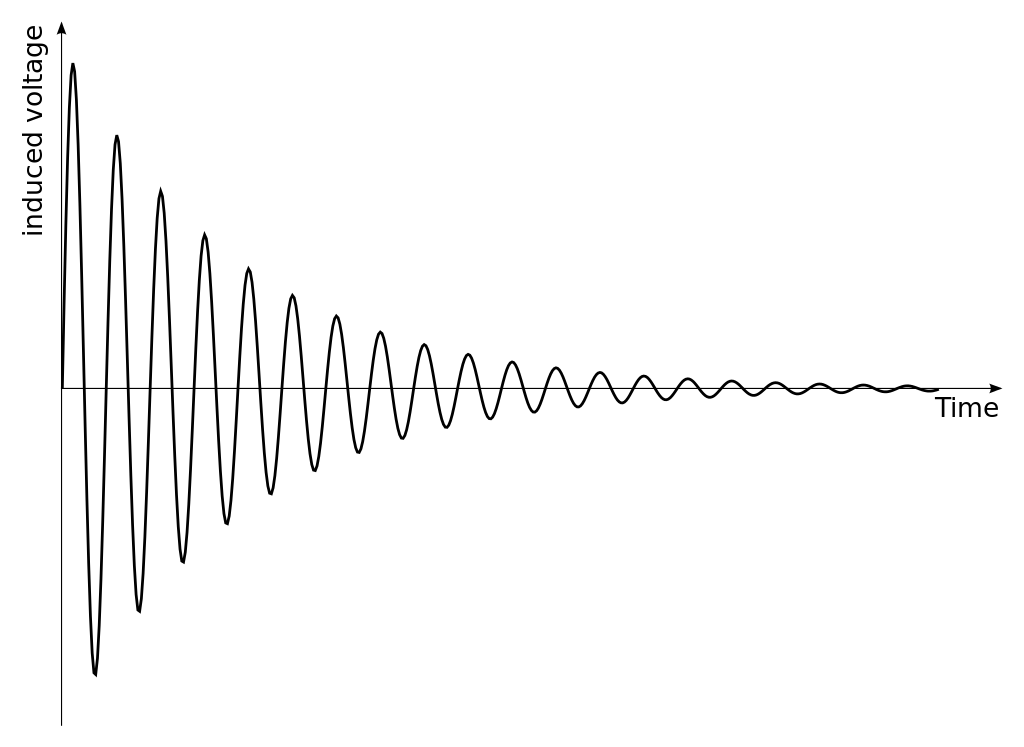
\includegraphics[width=0.6\textwidth]{Nmr_fid_good_shim_EN}
    \caption[FID signal]{An example FID signal. The current picked up in the coils around the proton sample will oscillate as the spins precess around the main magnetic field, and decay as the spins return to alignment with the external field.}
    \label{fig:FID}
\end{figure}

It is not solely $\omega_{p}$ that needs to be measured. What really matters is the average magnetic field that the muons see, namely the time-averaged spatially-weighted magnetic field. The scheme devised to measure this is two-fold. First, the magnetic field in the muon storage region is measured by a trolley which travels around the inside of the ring. This trolley holds 17 NMR probes which measure the field at approximately 6000 locations around the inside of the ring. However, because the trolley cannot be in the storage region when the muons are present in the ring, during data taking it is retracted and the field is instead monitored by 378 fixed NMR probes located in the high magnetic field region, just outside the storage region on the outside of the vacuum chambers. The prescription is that the storage ring field is measured every few days by the trolley probes, and the field between trolley runs is interpolated using measurements from the continually-sampling fixed probes. In this way the magnetic field can be mapped over time and over the space in which the muons are stored. A sample of the azimuthally-averaged magnetic field measured with trolley and fixed probes is shown in \figref{fig:AverageMagneticField}.

\begin{figure}
    \centering
    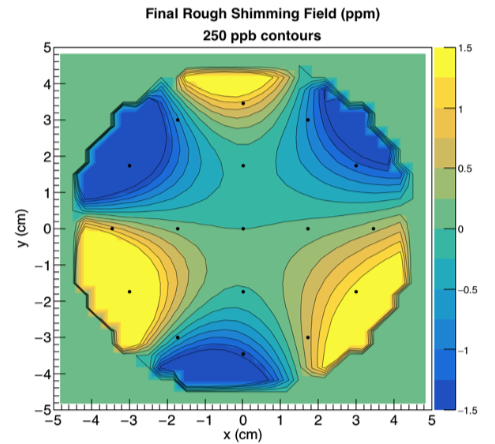
\includegraphics[width=0.7\textwidth]{MagneticFieldMapClean}
    \caption[Azimuthally averaged magnetic field sample]{A sample of the azimuthally-averaged magnetic field within the storage region courtesy of R. Osofsky \cite{fieldmap}. The contours are normalized to the field value at the center of the storage region. The scale of the field differences is approximately $\pm 1.5$~ppm. The black dots in the picture correspond to the location of the trolley probes.}
    \label{fig:AverageMagneticField}
\end{figure}


Lastly, it is the free proton precession frequency in the field that is of interest, but the frequency that the trolley probes measure will be different due to the molecular properties of the proton sample as well as the material properties of the probe itself. The frequency of the induction signal that the probes measure can be re-cast as 
        \begin{align} \label{eq:wpprobe}
            \omega_{p,\text{probe}} = \omega_{p,\text{free}}(1 - \sigma(\text{H\textsubscript{2}O, T}) + \delta_{b} + \delta_{p} + \delta_{s}),
        \end{align}
where $\sigma(\text{H\textsubscript{2}O, T})$ is the temperature-dependent diamagnetic shielding of protons in a water molecule, and the $\delta$'s come from corrections due to the bulk susceptibility of the water sample, paramagnetic impurities in the water sample, and the magnetic effects of the probe itself, respectively \cite{TDR}. In order to correct for these effects two additional special probes are used, both of which live in a single section of the ring which has been shimmed to extra uniformity. The first is a calibration probe which measures the free proton precession frequency at the center of the storage region, corresponding to the position of the central trolley probe. The calibration probe is made of materials which are designed to reduce the effects listed in \equref{eq:wpprobe}, and has been characterized in a dedicated highly uniform solenoidal magnetic field. The second special probe is called the `plunging probe.' This probe is located inside the vacuum chamber and moves into the storage region to measure the field at each of the 17 trolley probe locations, using a three dimensional motion system. By using these two probes, the calibration to the free proton precession frequency can be transmitted to each of the trolley probes, providing an absolute scale for the measurements inside the muon storage region. The uncertainty on the calibration procedure is estimated to be $\SI{35}{ppb}$, about half the total permitted by the experimental error budget of $\SI{70}{ppb}$.


Other pieces of the systematic uncertainty include the calibrations of the probes, errors in the trolley measurements, the interpolation with the fixed probes, the uncertainty of the magnetic field relative to the muon distribution, and others such as time dependent external magnetic fields, \tabref{tab:magneticfielduncertainties}.


\begin{table}
\centering
\setlength\tabcolsep{10pt}
\renewcommand{\arraystretch}{1.2}
\begin{tabular*}{.8\linewidth}{@{\extracolsep{\fill}}lc}
  \hline
    \multicolumn{2}{c}{\textbf{Magnetic Field Measurement Uncertainties}} \\
  \hline\hline
    Source of uncertainty & E989 Goal (ppb) \\
  \hline
    Absolute calibration of standard probe & 35 \\
    Calibration of trolley probes & 30 \\
    Trolley measurements & 30 \\
    Fixed probe interpolation & 30 \\
    Muon distribution weighted average & 10 \\
    Time dependent external fields & 5 \\
    Others & 30 \\
  \hline
    Quadrature sum & 70 \\
  \hline 
\end{tabular*}
\caption[Uncertainties in the magnetic field measurement]{Systematic errors in the magnetic field measurement. Unlisted sources of error include the measurement of higher field multipoles, trolley temperature and power supply voltage response effects, and eddy currents from the kicker, among others.}
\label{tab:magneticfielduncertainties}
\end{table}



\section{Production of polarized muons}
\label{sec:Accelerator}

% The Feynman diagram for this decay is shown in \figref{fig:pidecay}. 

As explained in \secref{section:WaIntro}, in order to measure \wa the muons injected into the storage ring must be polarized. The BNL E821 experiment observed on the order of 10 billion positrons above threshold, and its final result was statistics limited. In order to reach the goal of $\SI{140}{ppb}$, approximately 20 times that number of positrons needs to be gathered, and hence a large number of polarized muons produced. Fermilab has the facilities to produce such a large number of polarized muons.

Polarized muon beams are constructed using the physics of pion decay. Using the same parity-violation and spin momentum conservation logic as explained in the discussion of muon decay, it is determined that pion decay produces muons that are 100\% polarized in the pion rest frame, due to the pion having zero spin. It is also important to note that pions decay to muons with a $\sim 99.98\%$ branching ratio due to the parity violating nature of the weak interaction \cite{PDG}. Thus by producing a large number of polarized pions a large number of polarized muons can be acquired.


\begin{figure}
    \centering
    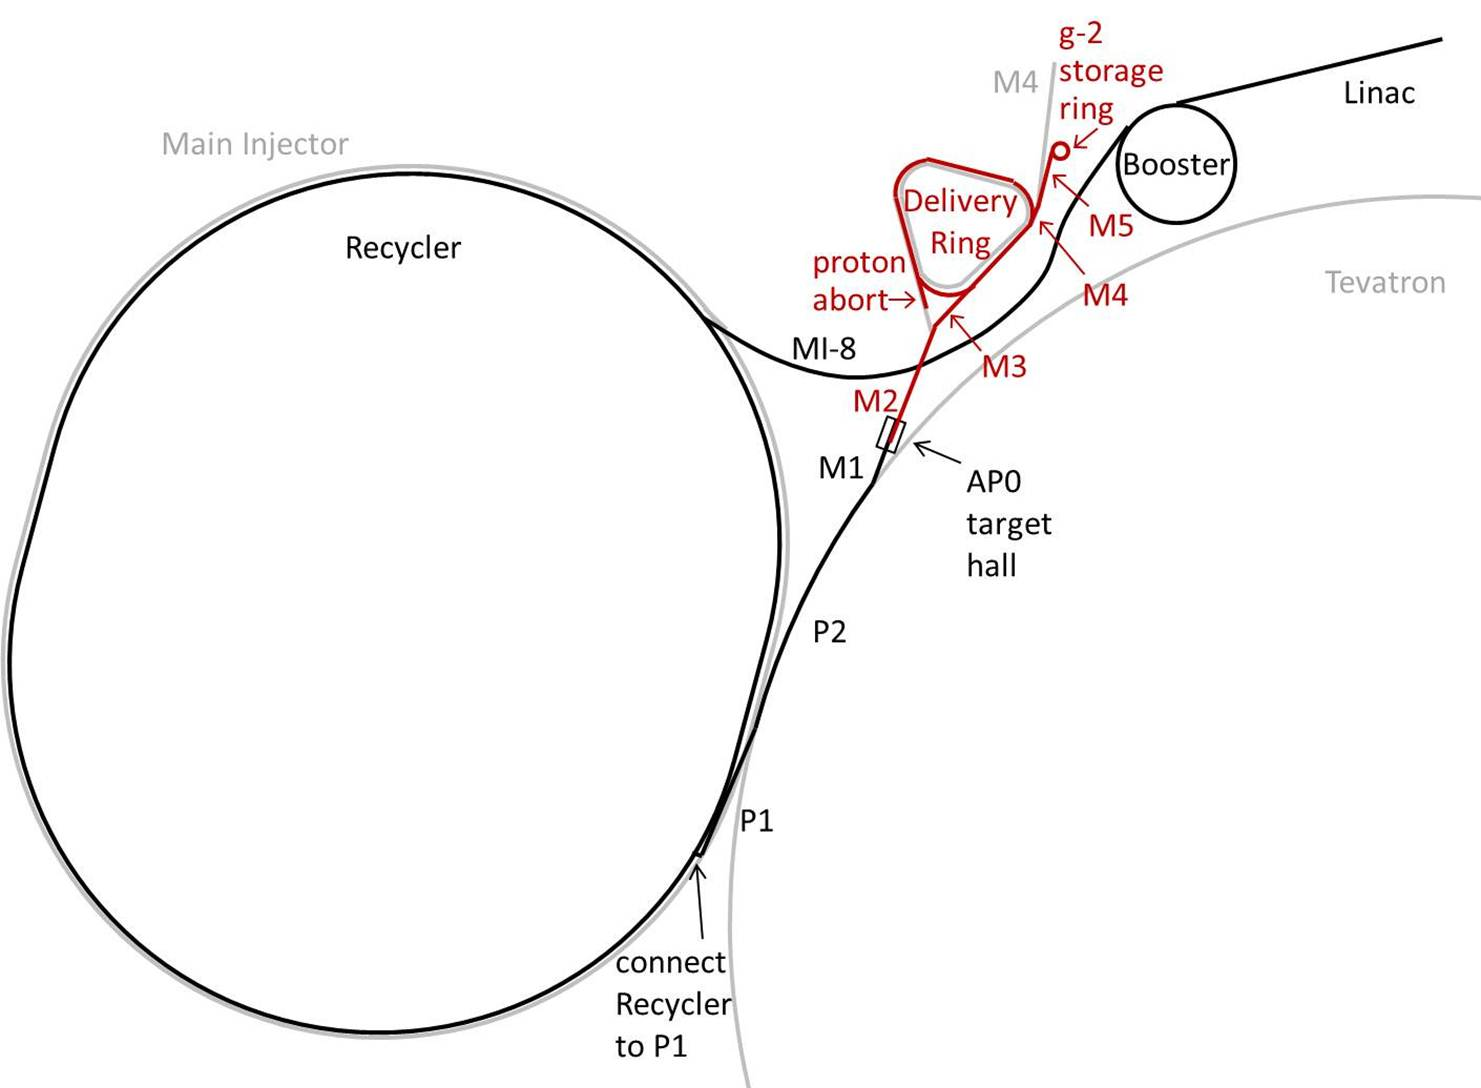
\includegraphics[width=1\textwidth]{accel_layout}
    \caption[Fermilab accelerator layout for muon delivery to E989]{The layout of accelerator beam-line components Fermilab uses to provide polarized muons to E989. Protons start in the Linac, traverse around the Booster and then Recycler, and are converted to pions at AP0. The pions are gathered and then decay to muons in the Delivery Ring before being sent to the \gmtwo storage ring. \cite{TDR}.}
    \label{fig:accelerator}
\end{figure}

The production of polarized muons for E989 at the Fermilab accelerator complex involves a number of stages. A map of the various relevant accelerator beam-line components is shown in \figref{fig:accelerator}. Details of the full accelerator production of polarized muons can be found in \refref{Stratakis:2017uci}, and here a summary of the process will be given. First, H\textsuperscript{-} ions are produced and accelerated in a linear accelerator. They are stripped down to protons and then transported to a $\SI{75}{m}$ radius circular storage ring called the ``booster,'' which accelerates them up to $\SI{8}{\GeV/c}$ and batches them together. A single booster batch contains on the order of $\SI{4e12}{protons}$. The protons are then injected into a ring called ``recycler,'' which separates them into four separate bunches of $\SI{1e12}{protons}$, each with a time width of approximately $\SI{120}{ns}$. (This is less than the cyclotron period of the storage ring of \SI{149}{ns}.) This re-bunching process is done in order to reduce the instantaneous rates observed by the detectors, and thus reduce the level of pileup in the E989 detectors; see \secref{sub:calosystematics}. For a single accelerator supercycle of $\SI{1.4}{s}$, E989 receives four booster batches corresponding to sixteen recycler bunches at an average rate of $\SI{11.4}{Hz}$, with the time separation between bunches greater than $\SI{10}{ms}$. The timing structure is shown in \figref{fig:pulsetrain}, where trains of eight bunches are sent to E989 with some time separation between them\footnote{These eight bunches are sometimes referred to as pulses, and the gathered data is tagged by which bunch or pulse it originates from.}. Although it remains relatively constant, this timing structure may be modified in response to the requirements of other experiments.

\begin{figure}
    \centering
    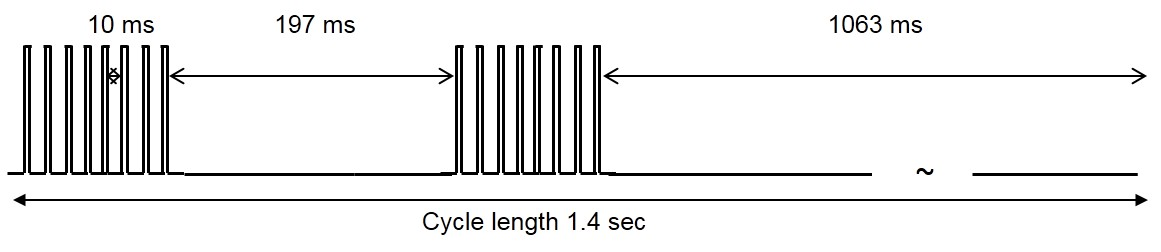
\includegraphics[width=1\textwidth]{accel_pulsetrain}
    \caption[Fermilab accelerator pulse train]{General timing structure of beam pulses sent to E989.}   
    \label{fig:pulsetrain}
\end{figure}


Each bunch is sent to a target hall, where it is directed on to an Inconel target. This Inconel target is made of a nickel-iron alloy, and is optimized for the production of a large number of pions with a small momentum spread, approximately $\SI{1e-5}{\pi^{+}}$ per proton on target with $|dp/p| < 2 \%$ \cite{Stratakis:2017uci}. The pions are focused by the magnetic field of a lithium lens, located just downstream of the production target. The lens, a cylinder of lithium $\SI{1}{cm}$ in radius and $\SI{15}{cm}$ long, carries a large current down its length which provides a radial focusing effect for particles passing down the cylinder \cite{LiLens}. A pulsed magnet just after the lithium lens is then used to select pions and residual particles, mainly protons, centered at $\SI{3.115}{\GeV}$.


The resultant pion beam and these residual particles are then injected into another ring called the ``delivery ring''\footnote{By the time the pions have gotten to the delivery ring, most of them have decayed to muons.}. Here it should be noted that in a pion beam the highest and lowest energy decay muons are forwards and backwards polarized, respectively. The delivery ring is used to momentum select polarized muons and separate out the non-desired particles which will have differing velocities compared to the muons, reducing the contamination in the final polarized muon beam \cite{Stratakis:2017uci}. Forward emitted polarized muons are momentum selected at their decay energies of $\SI{3.094}{\GeV}$ with $\Delta p / p = 2\%$. Particles that fall outside the momentum acceptance are lost, and the residual protons are kicked into a beam dump. The polarized muon beam is then sent to the E989 building where it passes through four magnetic quadrupole focusing magnets before being injected into the E989 storage ring.




\section{Injection of muons}
\label{sec:injection}


The injection of the muon beam into the E989 storage ring is a specialized process. In order to measure the magnetic field to the precision described in \secref{sec:MagneticField}, the storage ring must be a single monolithic magnet with no end effects. This prohibits the usual design of separated magnetic elements through which the muons might be injected. Therefore the beam must be injected through the storage ring magnet yoke. This introduces the design constraint where the main magnet field must be eliminated within the injection tunnel, such that muons are not lost due to deflection into the magnet itself. Any solution to this problem must have it's cancellation field localized to the injection tunnel, such that there is no residual fringe field that contaminates the main storage ring dipole field. 

A specialized magnet called the ``Superconducting Inflector'' magnet, or just inflector, is used to solve these design constraints. This inflector is placed just after a bored out tunnel in the storage ring magnet yoke, on the inside of the C shape. See \figref{fig:injectionpoint} for a view of the injection point. The inflector has an $\SI{18}{mm}$ wide by $\SI{56}{mm}$ high aperture through which the muons must pass down its $\SI{1.7}{m}$ length. The inflector is made up of superconducting coils wrapped in a truncated double cosine theta design around an aluminum mandrel \cite{inflector}. See \figref{fig:inflector}. This design serves to contain the majority of the inflector magnet field, while eliminating the the storage ring field for the muons passing down its length. The inflector is contained within a superconducting shield which traps the fringe field of the inflector such that the storage ring magnet field is unaffected. As shown in \figref{fig:inflector}, windings cover both ends of the inflector such that an appreciable fraction of muons are lost due before being injected into the ring. In order to increase the muon flux for future runs of E989, a new inflector magnet is being designed with open ends \cite{TDR}.


\begin{figure}
    \centering
    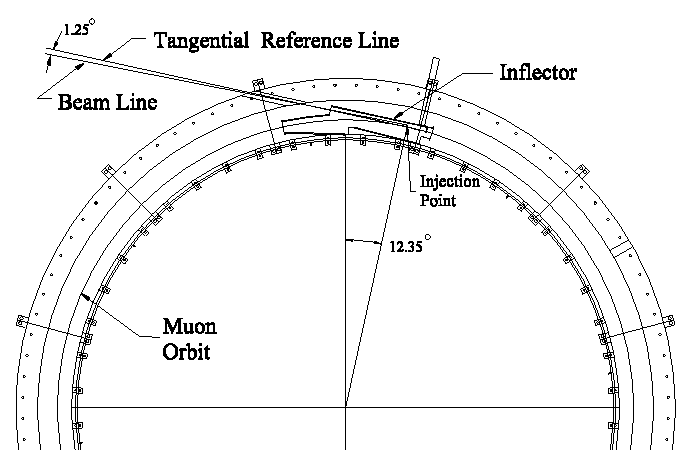
\includegraphics[width=.7\textwidth]{injectionpoint}
    \caption[Muon injection point through inflector]{A plan view of the inflector and injection point into the storage ring \cite{inflector}.}   
    \label{fig:injectionpoint}
\end{figure}

\begin{figure}
\centering
    \begin{subfigure}[t]{0.45\textwidth}
        \centering
        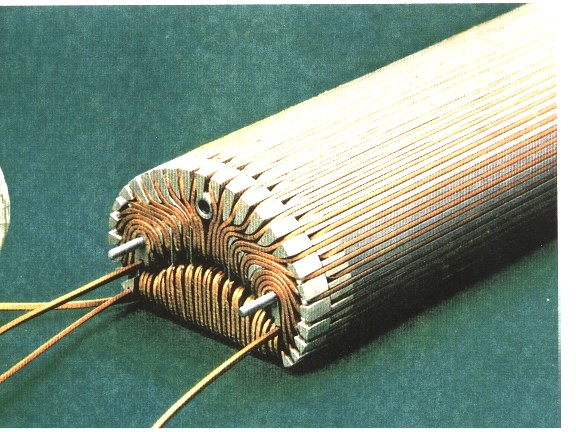
\includegraphics[width=\textwidth]{inflector_closed}
        \caption{End view of the inflector.}
    \end{subfigure}%
    \hspace{1cm}
    \begin{subfigure}[t]{0.45\textwidth}
        \centering
        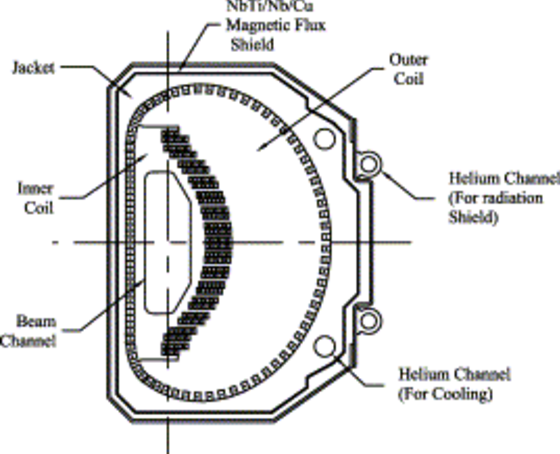
\includegraphics[width=\textwidth]{inflectorcrosssection}
        \caption{Cross section view of the inflector.}
    \end{subfigure}
\caption[Superconducting inflector magnet]{The inflector magnet (left) and a cross section view of the inflector windings and associated shield (right) \cite{inflector}.}
\label{fig:inflector}
\end{figure}



\section{Storage of muons}
\label{sec:Storage}

\begin{figure}
    \centering
    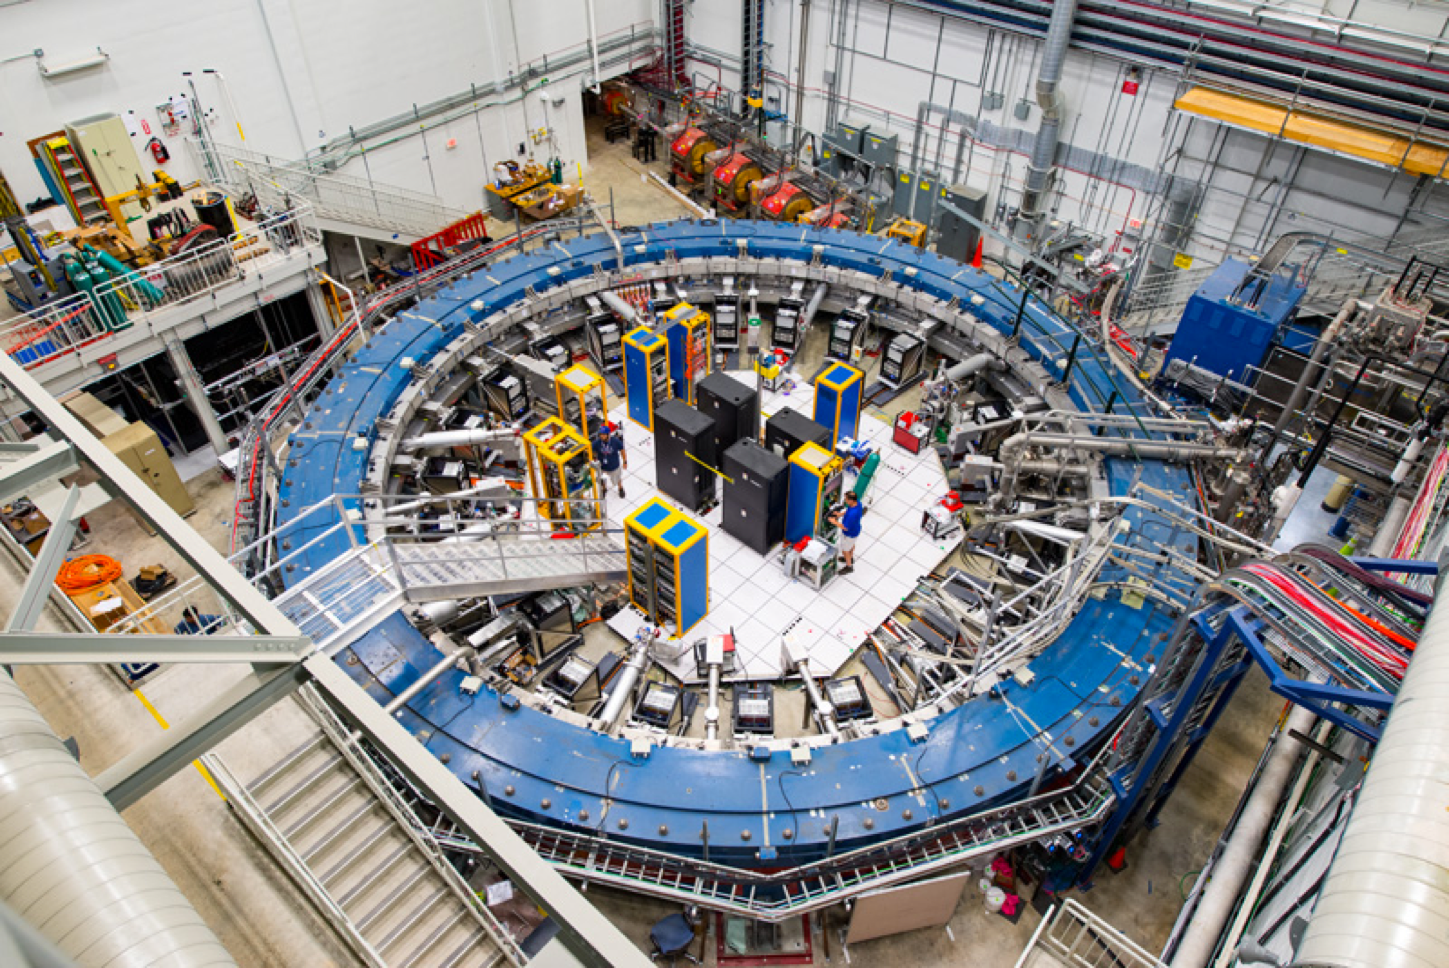
\includegraphics[width=1\textwidth]{ring}
    \caption[The E989 experiment]{The E989 experiment. The blue storage ring can be seen to surround a variety of detectors and electronics. Muons from the accelerator enter at the top of the picture, and are transported to the storage ring through a series of magnetic quadrupoles. Muons are injected through the inflector into the ring, where they orbit in a clockwise direction. The ring is approximately $\SI{16}{m}$ in diameter to the outside edge of the ring, and about $\SI{3}{m}$ high. People in the center of the ring give a sense of scale to the picture.}
    \label{fig:ring}
\end{figure}


Once the muons have been injected into the ring, they will begin orbiting clockwise around the ring, decaying with a lifetime of $\SI{64.4}{\micro s}$.  The E989 experiment and storage ring are shown in \figref{fig:ring}. By necessity, the inflector must be out of the stored muon beam path, otherwise a large fraction of the muons would be lost upon the return to the injection point as the muons would strike the inflector. Therefore the muon beam must be kicked to move the beam path from the injection orbit onto the central orbit of the storage ring. The muon beam must also be contained vertically. To perform the former, a magnetic ``kicker'' is used to shift the orbits of the muons. To perform the latter, a series of electrostatic quadrupoles focus the beam vertically. Approximately 2\% of the injected muons are stored with $\Delta p / p = 0.1\%$ centered around $\SI{3.094}{\GeV/c}$, corresponding to a design goal of $\mathcal{O}(10,000)$ stored muons per fill.


\subsection{Kicker}
\label{sub:kicker}

The kicker is made up of three separate pulsed magnets located 90\textdegree{} from the exit of the inflector, where the injection orbit crosses the central orbit. The placement of the kickers is shown in \figref{fig:vacmap}. The kicker must be located within the precision magnetic field of the ring, and must therefore contain no magnetic elements in the hardware itself. For this reason each kicker magnet is made up of two thin $\SI{1.27}{m}$ long aluminum plates, separated by $\SI{10}{cm}$, which carry the current used to create the kicking magnetic field. Due to the bunched nature of the muon beam and the short cyclotron period of $\SI{149}{ns}$, ideally the kicker moves all injected muons onto the central orbit and then turns off quickly such that by the time the muons orbit back around to the kicker there is no residual kick to the beam. Any residual eddy currents must die away quickly enough such that the magnetic field seen by the stored muons is unperturbed. The design deflection of the beam is approximately $\SI{10}{mrad}$ using a vertical pulsed field of around $\SI{300}{Gauss}$ (corresponding to kicker plate voltages of $\mathcal{O(\SI{155}{kV})}$) with a pulse length of about $\SI{120}{ns}$ \cite{TDR}. The operational kicker performance in Run 1 was less, as described in \secref{sec:Run1}.


%A picture of one of the kickers installed into the vacuum chamber is shown in 

\begin{figure}
    \centering
    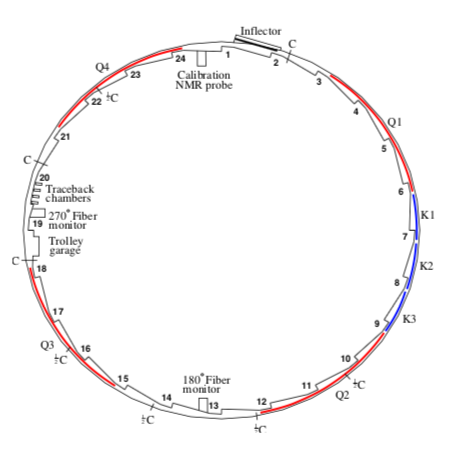
\includegraphics[width=\textwidth]{VacuumChamberMap}
    \caption[Vacuum chamber map]{A map of the vacuum chambers in E989. K1-K3 show the locations of the kicker magnets, while Q1-Q4 show the locations of the electrostatic quadrupoles. Also shown is the location of the inflector, the two fiber monitors, and one of the tracker stations.}   
    \label{fig:vacmap}
\end{figure}

\subsection{Electrostatic quadrupoles}
\label{sub:quads}

There are four electrostatic quadrupoles located around the ring as shown in \figref{fig:vacmap}, which provide vertical focusing for the beam. Although the quadrupoles are defocussing in the horizontal plane, the main dipole magnetic field provides net horizontal focusing. Just as with the kickers, the quadrupoles must be operated in vacuum. E989 uses electrostatic focusing elements instead of magnetic ones in order to avoid magnetic field gradients which would limit the precision of the magnetic field measurement. The quadrupoles occupy 43\% of the ring circumference, with four quads having been chosen in order to maximize the symmetry of the beam motion, reduce its amplitude, and leave space for other experimental elements around the ring \cite{TDR}. Each quadrupole is made up of two segments, a short segment of 13\textdegree{} and a long segment of 26\textdegree{} corresponding to $\SI{1.61}{m}$ and $\SI{2.62}{m}$ respectively, with each segment consisting of four plates. To minimize multiple scattering of incident decay positrons, the quadrupoles are made as thin as possible. A picture of the quadrupoles installed into one of the vacuum chambers is shown in \figref{fig:Quads}. A calculation of the equipotential lines of the quadrupoles is shown in \figref{fig:QuadPotential}. The original design of the quadrupoles is detailed in \refref{QuadsE821}.

\begin{figure}
    \centering
    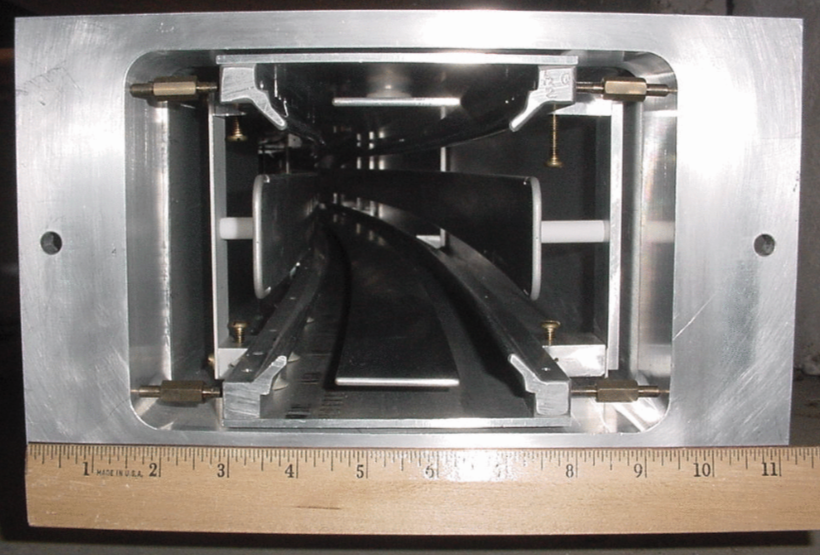
\includegraphics[width=.7\textwidth]{Quads}
    \caption[Electrostatic quadrupoles installed in a vacuum chamber]{Electrostatic quadrupoles installed into a vacuum chamber \cite{QuadsE821}. There are four plates mounted to the chamber through insulator standoffs, with the distance between opposing quadrupole plates equal to $\SI{10}{cm}$. Also shown are the rails on which the magnetic field trolley rides. Note that as the trolley makes its way through the storage volume, it must pass between both the various sets of quadrupole and kicker electrodes.}
    \label{fig:Quads}
\end{figure}

\begin{figure}
    \centering
    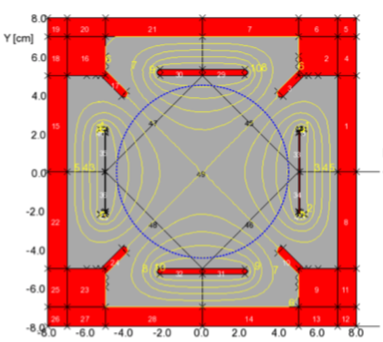
\includegraphics[width=.6\textwidth]{QuadPotential}
    \caption[Electrostatic quadrupole potentials]{An OPERA model of the quadrupoles and their equipotential contours \cite{TDR}. The top and bottom plates sit at positive voltage while the left and right plates are at negative voltage. The muon storage region is shown by the blue circle.}   
    \label{fig:QuadPotential}
\end{figure}


Some of the stored muons will be lost during data taking that can adversely affect the measurement of the spin difference frequency \wa. See \secref{subsec:lostmuons}. In order to reduce the number of lost muons, a procedure called ``scraping'' is used to remove those muons sitting at the edge of the storage region that are more likely to be lost at later times. This scraping procedure involves powering the quadrupole voltages in an asymmetric way such that the beam is pushed to the outside of the storage region, where the edges of the beam will intersect copper collimators. These collimators have a radius of $\SI{45}{mm}$ and define the storage region aperture. Muons which hit the collimators will lose energy and be lost as they spiral out of the ring. The scraping procedure is performed early in the fill and ends at \mus{8}, such that by \mus{30} the beam is stable and centered due to the characteristic RC time constant of the system. The operational performance of the quadrupoles in Run 1 is described in \secref{sec:Run1}, where it was found that the quads had a longer RC time constant than the design.



\section{Muon beam dynamics}
\label{sec:muonbeamdynamics}

Muons injected into the storage ring will occupy a region in phase space of momenta and positions defined by the injection and collimator apertures. Individual muons will undergo betatron motion within the storage ring in both the vertical and horizontal directions. The horizontal ($x$) and vertical ($y$) equations of motion, including the effects of the discrete quadrupoles, are given by
        \begin{align} \label{eq:betatronmotion}
            x &= x_{e} + A_{x}(s) \cos(\nu_{x} \frac{s}{R_{0}} + \phi_{x}), \\
            y &= A_{y}(s) \cos(\nu_{y} \frac{s}{R_{0}} + \phi_{y}), 
        \end{align}
where $x_{e}$ is the radial equilibrium orbit of the beam relative to $R_{0}$, $A_{x}(s)$ and $A_{y}(s)$ are the amplitudes of the motions containing the effects of the discreteness of the quadrupoles, and $s$ is the arc length of the trajectory. Here $\nu_{x}$ and $\nu_{y}$ are the so-called horizontal and vertical ``tunes'' of the beam motion, which are ratios of the betatron frequencies to the cyclotron frequency $f_{c}$: 
        \begin{equation} \label{eq:tunes}
        \begin{aligned}
            \nu_{x} &= f_{x_{BO}}/f_{c} = \sqrt{1-n} \\
            \nu_{y} &= f_{y_{BO}}/f_{c} = \sqrt{n}
        \end{aligned}
        \end{equation}
These are related to the field index $n$, where the field index characterizes the strength of the electrostatic focusing in relation to the magnetic field strength: 
        \begin{align} \label{eq:fieldindex}
            n = \frac{\kappa R_{0}}{\beta B_{0}},
        \end{align}
where $\kappa$ is the electric quadrupole gradient, $B_{0}$ is the magnetic field strength, $R_{0}$ is the central storage ring radius, and $\beta \cdot c$ is the velocity of the muon beam. Technically $n$ is the the average field index around the ring, where this approximation is justified due to the four-fold symmetry of the discrete quadrupoles and the fact that the betatron oscillations have wavelengths much greater than the length of the quads. A table of the important frequencies in E989 is shown in \tabref{tab:frequencies}. Lastly, the maximum angular acceptance of the ring can be determined from the betatron oscillations and the field index as 
        \begin{equation} \label{eq:maxangles}
        \begin{aligned}
            \psi_{x_{max}} &= \frac{x_{max}\sqrt{1-n}}{R_{0}}, \\
            \psi_{y_{max}} &= \frac{y_{max}\sqrt{n}}{R_{0}},
        \end{aligned}
        \end{equation}
where $x_{max}$ and $y_{max}$ are both equal to the radius of the storage region aperture at $\SI{45}{mm}$.


\begin{table}
\centering
\setlength\tabcolsep{10pt}
\renewcommand{\arraystretch}{1.2}
\begin{tabular*}{1\linewidth}{@{\extracolsep{\fill}}lcccc}
  \hline
    \multicolumn{5}{c}{\textbf{Muon Beam Frequencies}} \\
  \hline\hline
    Name & Symbol & Expression & Frequency (MHz) & Period \\
  \hline
    \gmtwo & $f_{a}$ & $a_{\mu}Be/2\pi m c$ & 0.23 & $\SI{4.365}{\micro s}$ \\
    cyclotron &  $f_{c}$ & $v/\pi R_{0}$ & 6.71 & $\SI{149.2}{ns}$ \\
    horizontal betatron & $f_{x_{BO}}$ & $\sqrt{1-n} f_{c}$ & 6.34 & $\SI{158}{ns}$ \\
    vertical betatron & $f_{y_{BO}}$ & $\sqrt{n} f_{c}$ & 2.21 & $\SI{452}{ns}$ \\
    coherent betatron & $f_{CBO}$ & $f_{c}-f_{x_{BO}}$ & 0.37 & $\SI{2.703}{\micro s}$ \\
    vertical waist & $f_{VW}$ & $f_{c}-2f_{y_{BO}}$ & 2.31 & $\SI{433}{ns}$ \\
  \hline
\end{tabular*}
\caption[Muon beam frequencies in the E989 experiment]{Frequencies seen in the \gmtwo experiment due to beam motion. Parameter values are from a subset of Run 1 corresponding to an $n$ value of 0.108 or a quadrupole voltage of 18.3 kV.}
\label{tab:frequencies}
\end{table}


As the muon beam goes around the ring, the muons will experience local field gradients and inhomogeneities. The muons will inevitably pass through the perturbations many times. However, if they don't pass through the perturbations at the same phases of their betatron motion, the amplitude of the would-be resonant oscillation won't continue to grow. The tunes are chosen to avoid these resonances by having the muons sample the entire azimuth of the ring equally, thus keeping the beam stored. The general resonance condition is \cite{Wiedermann}
        \begin{align}
            a \nu_{x} + b \nu_{y} = c,
        \label{eq:tunecondition}
        \end{align}
where $a$, $b$, and $c$ are integers. We know from \equref{eq:tunes} that 
        \begin{align}
            \nu_{x}^{2} + \nu_{y}^{2} = 1,
        \label{eq:tuneone}
        \end{align}
which constrains the available $n$ values that can be chosen. \figref{fig:tuneplane} shows the intersections of the resonant lines of \equref{eq:tunecondition} along with the circular arc of \equref{eq:tuneone} in the tune plane, for which a chosen value of $n$ will lie on a resonance. The operational $n$ values and corresponding quadrupole voltages in Run 1 are described in \secref{sec:Run1}.

% Moved to Run1 section
% For Run 1 data taking, $n$ values of 0.108 and 0.120 were chosen corresponding to quadrupole voltages of 18.3 and $\SI{20.4}{kV}$ respectively \cite{tunetable}. The associated betatron wavelengths are 1.06 and 3.04 times the circumference of the storage ring respectively.


\begin{figure}
    \centering
    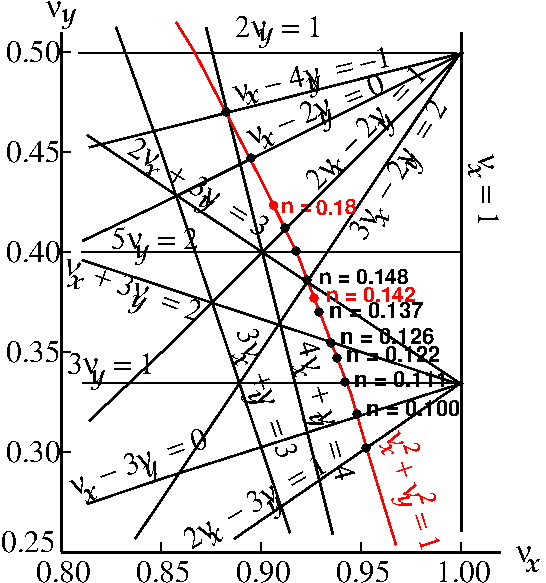
\includegraphics[width=.5\textwidth]{tuneplane}
    \caption[Tune plane]{The tune plane, with the $\nu_{x}^{2} + \nu_{y}^{2} = 1$ constraint in red. The chosen value of $n$ lies on this circle. The original design goals for E989 were the $n$ values as shown by the red points, but due to hardware issues smaller $n$ values of 0.108 and 0.120 were chosen as described in \secref{sec:Run1}.}
    \label{fig:tuneplane}
\end{figure}



\subsection{Coherent betatron oscillation}
\label{sub:CBO}

The muon beam consists of many muons, each individually undergoing betatron oscillations. If the phase of the oscillations of the individual muons are incoherent, then the beam can be thought of as a static entity, constant in time around the ring. However, due to injection and kicker effects which induce a particular phase space distribution on the injected beam, the beam itself can be said to oscillate. The beam is then described by a width and mean dependent on the injection process, and the strength and phase of the kicker pulse, such that the phase distribution of the beam oscillates coherently every betatron wavelength\footnote{The four-fold quadrupole symmetry was chosen in order to minimize this beam `breathing.'}. Due to the mismatching of betatron wavelengths to the ring circumference in order to avoid resonances, a singular time slice of the distribution can be said to move around the ring over time. Individual detectors around the ring measure the beam in discrete pieces based on their individual azimuthal acceptances, where these acceptances depend on the radial and vertical characteristics of the beam. Because the radial betatron frequency is larger than half the cyclotron frequency, there is an aliasing effect such that the radial betatron motion of the beam is instead observed as an apparent slow-moving oscillation. We call the measurable signal of this coherent radial motion coherent betatron oscillation (CBO). See \figref{fig:cbo} for a pictorial view of this phenomenon. Since the acceptance of the calorimeters depend on the beam properties, the CBO will modulate the \wa signal.

The frequency of the CBO is just the beat frequency between the cyclotron frequency and the horizontal betatron frequency
        \begin{align} \label{eq:CBOfreq}
            f_{CBO} = f_{c}-f_{x_{BO}}.
        \end{align}
There is also a vertical CBO effect, but the non-aliased rate of oscillation is fast enough such that the effect tends to average out. However, the detectors are sensitive to oscillations of the vertical width of the beam, which is aliased in a similar way to the radial oscillation. Though the principles are the same, we call this effect the vertical waist (VW),
        \begin{align} \label{eq:VWfreq}
            f_{VW} = f_{c}-2f_{y_{BO}},
        \end{align}
where the term \textit{waist} refers to the minimum vertical width. Both of these frequencies are included in \tabref{tab:frequencies}. The phase of the CBO signal varies systematically by detector, from 0 \SIrange{0}{2\pi}{} around the ring. When adding all of the detector signals together, the CBO oscillations tend to cancel out. However, due to acceptance differences between the different detectors, the CBO oscillations are still observable in the data. When fitting the data to extract \wa, these effects must be accounted for in the fit function, as will be discussed in \secref{sub:cboterms}.


\begin{figure}
    \centering
    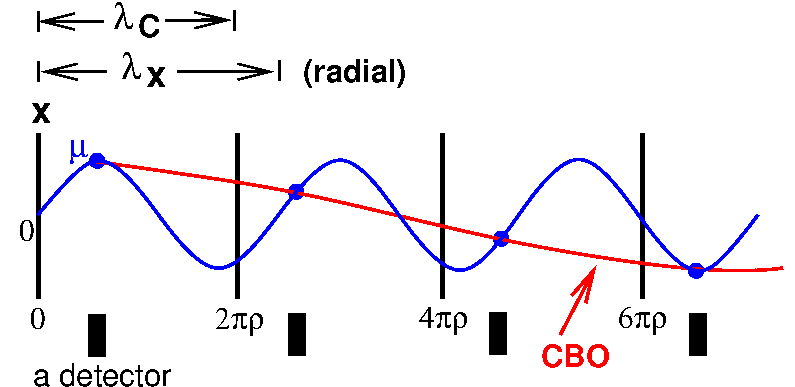
\includegraphics[width=.6\textwidth]{cbo}
    \caption[Coherent betatron oscillation]{Marked by the black vertical lines are integer steps in the circumference of the ring, corresponding to the cyclotron wavelength $\lambda_{c}$. The blue line shows the motion of the beam due to the betatron oscillations $\lambda_{x}$. Since $\lambda_{x} > \lambda_{c}/2$, there is an aliasing effect in the observed signal, which is identified by the red line. To a single detector the beam appears to move slowly back and forth with $f_{CBO}$.}
    \label{fig:cbo}
\end{figure}


\subsection{Beam debunching}
\label{sub:beam_debunching}

As described in Sections~\ref{sec:Accelerator} and \ref{sec:injection}, the muon beam is injected into the ring with a time spread of $\SI{120}{ns}$ and a range of momenta. At early times the beam will occupy a portion of the ring less than the whole since the cyclotron period is $\SI{\sim149}{ns}$. At initial injection, detectors located at discrete points around the ring see a high intensity as the beam passes by and low intensity when it is on the other side of the ring. The cyclotron period of each muon is determined by its particular momentum which gives its radius of orbit. Higher momentum muons have a larger radius and therefore larger distance to travel, thus taking longer to circulate the ring than lower momentum muons. This leads to the low momentum muons in the head of the bunch catching up with the high momentum muons in the tail, such that the gaps in between each passing of the beam bunch are reduced. By \mus{30} the muon beam has gone around the ring two hundred times and the gaps with no beam have reduced so much that the intensity is near-uniform. The varying intensity from the beam bunching is referred to as the ``fast rotation'' signal. This debunching signal is seen in the data as shown in \figref{fig:fastrotation}. When dealing with the data and attempting to extract \wa, the typical procedure is to both bin out the fast rotation in periods of the cyclotron frequency, and to randomize each hit time by $\pm T_{c}/2$ where $T_{c}$ is the cyclotron period. In this way the fast rotation is removed entirely and the effect can be ignored in the fitting procedure for \wa.


\begin{figure}
    \centering
    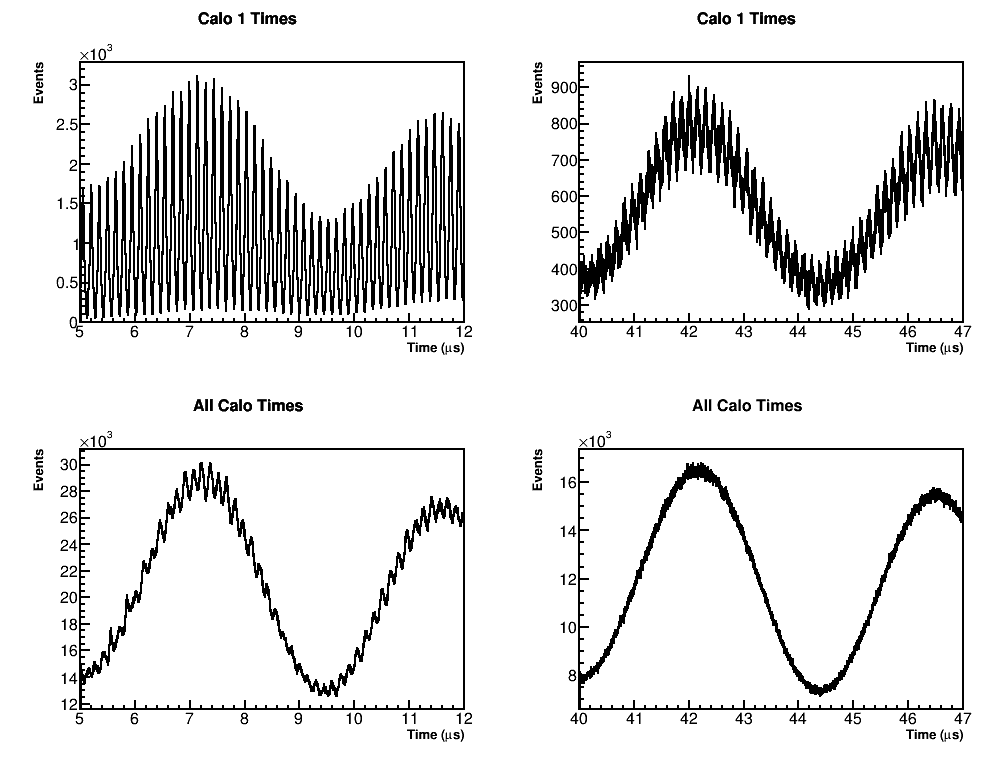
\includegraphics[width=\textwidth]{fastrotation}
    \caption[Beam debunching fast rotation]{In the data, the fast rotation signal is a fast ($\SI{149.2}{ns}$) modulation on top of the slower ($\mus{4.365}$) \wa frequency. The plots here are from a subset of data from Run 1. In individual calorimeters at early times the fast rotation signal is seen to be very large, as shown on the top left. As time passes and the beam debunches, the amplitude of the fast rotation signal diminishes as shown on the top right. When adding all calorimeters together, the signal is reduced as shown in the bottom two plots, due to the fast rotation signal being unaligned in phase for the different detectors.}
    \label{fig:fastrotation}
\end{figure}



\section{Corrections to \texorpdfstring{\wa}{wa}}
\label{sec:corrections}

\equref{eq:wasimple} is an idealized version of the spin difference frequency which ignores two important beam dynamics effects: torques exerted by the electric field and changes in the rest frame magnetic field resulting from the vertical pitching motion of the muons. Including practical experimental concerns, these two corrections must be applied to \wa.


\subsection{Electric field correction}
\label{sub:electric_field_correction}

In the presence of an electric field, the spin difference frequency is altered to 
        \begin{align} \label{eq:waelectric}
            \vec{\omega}_{a} = -\frac{q}{m} [a\vec{B} - \Big(a - \frac{1}{\gamma^{2}-1}\Big)(\vec{\beta} \times \vec{E}) ],
        \end{align}
where now there is an extra term dependent on the electric field strength and the momentum of the particles. This extra term originates from the motional magnetic field $\vec{\beta} \times \vec{E}$ that relativistic particles experience in an electric field. This is necessary to include since we use electrostatic quadrupoles for vertical focusing as described above.  The second term cancels to first order for a specific momentum or value of $\gamma$. This ``magic momentum'' can be understood as the momentum at which a relativistic particle moving through an electric field has its spin exactly follow its momentum. This magic momentum is $\SI{3.094}{\GeV}$ for muons, hence the momentum value of the injected muons. This value sets the energy and time scales of the experiment and has driven many of the design constraints, including the size of the storage ring, choice of the magnetic field magnitude, etc.

Not all muons will have the magic momentum however as described in the \secref{sub:beam_debunching}, and therefore a correction to the measured \wa frequency needs to be applied. Approximating the storage ring as having an electric field applied over the whole azimuth of the ring, the spin difference frequency for muons with momentum $p \neq p_{m}$ (where $p_{m}$ is the magic momentum) becomes  
        \begin{align} \label{eq:waEfield}
            \omega_{a}' = \omega_{a} \Big[ 1 - \beta \frac{E_{r}}{c B_{y}} \Big( 1 - \frac{1}{a \beta^{2} \gamma^{2}} \Big) \Big].
        \end{align}
Here the motion of the beam is assumed purely azimuthal. This additional term is the electric field correction that then serves to lower the measured \wa frequency. Using the relation $p = \beta \gamma m = (p_{m} + \Delta p)$, after a little bit of simplification the electric field correction can be written as
        \begin{align}
            C_{\text{E}} = \frac{\Delta\omega_{a}}{\omega_{a}} = -2 \frac{\beta E_{r}}{c B_{y}} \frac{\Delta p}{p_{m}}.
        \end{align}
The last fraction can be related to the field index described in \equref{eq:fieldindex} by
        \begin{align}
            \frac{\Delta p}{p_{m}} = (1-n) \frac{\Delta R}{R_{0}} = (1-n) \frac{x_{e}}{R_{0}}, 
        \end{align}
since we know that the magic momentum muons are at the central radius $R_{0}$ of the storage ring. In this equation $x_{e} = \Delta R$ is the equilibrium radius of the muon relative to the central storage radius. Noting that the radial electric field strength for a quadrupole is 
        \begin{align}
            E = \kappa x = \frac{n \beta c B_{y}}{R_{0}} x,
        \end{align}
and assuming that it is perfectly radial, the electric field correction reduces to 
        \begin{align}
            C_{\text{E}} = -2n (1-n) \beta^{2} \frac{x x_{e}}{R_{0}^{2}}.
        \end{align}
Taking the time average of the beam motion, where $x$ is simply equal to $x_{e}$, the correction becomes
        \begin{align}
            C_{\text{E}} = -2n (1-n) \beta^{2} \frac{\langle x_{e}^{2} \rangle}{R_{0}^{2}}.
        \end{align}
Since the equilibrium radius of the beam is set by the momentum distribution of the muons, this electric field correction can be determined by a measurement of the momentum spread of the beam which comes from an analysis of the fast rotation \cite{fastrotation1,fastrotation2}. For the precision goal of E989, the assumptions made in this derivation are acceptable \cite{TDR} and results will be cross-checked with spin-tracking simulations as was done in E821 \cite{E821FinalReport}. In E821 the electric field correction was approximately $\SI{500}{ppb}$ on \wa \cite{E821FinalReport}. In E989 the scale of the correction will be the same considering the experimental principles are identical, \secref{sub:EfieldPitchErrors}.


% Small corrections to the electric field correction due to the non-linearity and non-uniformity of the quadrupoles, as well as the assumptions made in this derivation, are discussed in \refref{}.



\subsection{Pitch correction}
\label{sub:pitch_correction}

Particles injected into the \gmtwo storage ring will have a vertical component of momentum which is parallel to the magnetic field vector (hence the need for vertically focusing electrostatic quadrupoles). This will slightly reduce the magnetic field seen by the muons in their rest frame. Including this motion into the spin difference frequency, \wa becomes
        \begin{align} \label{eq:wapitch}
            \vec{\omega}_{a} = -\frac{q}{m} [a\vec{B} - a \Big(\frac{\gamma}{\gamma+1}\Big)(\vec{\beta} \cdot \vec{B})\vec{\beta}],
        \end{align}
where now there is an extra term dependent on the vertical betatron motion of the beam. Similar to the electric field case, this term can be neglected to first order as the muon momentum is nearly all perpendicular to the field, but a correction again needs to be applied to \wa to account for this effect.

\begin{figure}
    \centering
    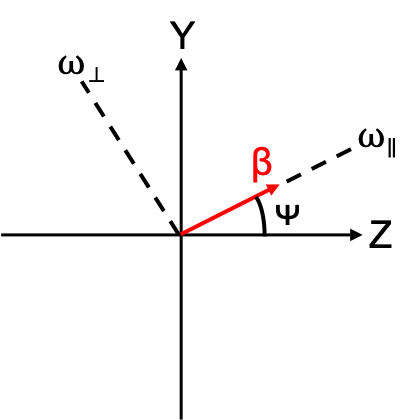
\includegraphics[width=.3\textwidth]{PitchAxes}
    \caption[Pitching beam motion]{Beam motion $\beta$ relative to the vertical and azimuthal axes Y and Z respectively. $\psi$ is the pitch angle of the beam, and the dashed lines represent the parallel and perpendicular motions of the beam.}   
    \label{fig:PitchAxes}
\end{figure}

Since the muons in the storage ring will be oscillating vertically as they are focused by the quadrupoles, their momentum vectors will be pitching up and down relative to the azimuthal motion. This pitch angle will oscillate as
        \begin{align} \label{eq:psi}
            \psi = \psi_{0} \cos(\omega_{y}t),
        \end{align}
where $\psi_{0}$ is the amplitude of the oscillation and $\omega_{y}$ is the vertical betatron frequency. Shown in \figref{fig:PitchAxes} is an exaggerated example of the beam motion relative to the vertical and azimuthal axes. Assuming that the field is purely vertical, $\vec{B} = B_{y}\hat{y}$ and that the beam motion is in the vertical-azimuthal plane,
        \begin{align}
            \vec{\beta} = \beta_{y}\hat{y} + \beta_{z}\hat{z} = \beta\sin(\psi)\hat{y} + \beta\cos(\psi)\hat{z},
        \end{align}
then \wa becomes
        \begin{align}
            \vec{\omega}_{a} = -\frac{q}{m} [a B_{y} \hat{y} - a \Big(\frac{\gamma}{\gamma+1}\Big) \beta_{y}B_{y} (\beta\sin(\psi)\hat{y} + \beta\cos(\psi)\hat{z})].        
        \end{align}
Using the small angle approximation such that $\cos(\psi) \approx 1$ and $\sin(\psi) \approx \psi$, $\vec{\omega}_{a}$ can be separated into its vertical and azimuthal components
        \begin{align}
            \omega_{ay} &= \omega_{a}\Big[ 1 - \Big(\frac{\gamma-1}{\gamma}\Big) \psi^{2} \Big], \\     
            \omega_{az} &= -\omega_{a} \Big(\frac{\gamma-1}{\gamma}\Big) \psi.
        \end{align}
Looking at \figref{fig:PitchAxes} again, it can be seen that the spin difference frequency can be resolved into its parallel and perpendicular components $\omega_{\parallel}$ and $\omega_{\perp}$ respectively. As the pitch angle of the beam motion oscillates about the azimuthal axes at a frequency much greater than the \gmtwo frequency, it can be seen that the parallel component averages to 0 over time. We then only care about the perpendicular oscillation of the beam, which can be determined with a simple rotation matrix such that
        \begin{align}
            \omega_{a} \approx \omega_{\perp} = \omega_{ay} \cos(\psi) - \omega_{az}\sin(\psi) \approx \omega_{a} \Big[ 1 - \frac{\psi^{2}}{2} \Big],
        \end{align}
where in the last approximation the small angle approximation was used once again, but this time with $\cos(\psi) \approx 1 - \psi^{2}/2$. The pitch correction then is the additional term which serves to lower the measured spin difference frequency. Taking the time average,
        \begin{align}
            C_{\text{P}} = \frac{\Delta\omega_{a}}{\omega_{a}} = - \frac{\langle \psi^{2} \rangle}{2}.
        \end{align}
The pitch angle of the beam cannot be measured directly, however we know from \equref{eq:maxangles} that the angle of the beam can be related to the vertical distribution of the beam, such that 
        \begin{align}
            C_{\text{P}} = - \frac{n}{2} \frac{\langle y^{2} \rangle}{R_{0}^{2}},
        \end{align}
where once again $n$ is the field index, $R_{0}$ is the radius of the ring at the center of the storage region, and $\langle y^{2} \rangle$ is the vertical width of the beam. The first two are known and the last can be measured experimentally by the straw tracking detectors. Just as in the case of the electric field correction, the assumptions made in this derivation are acceptable for the precision goal of E989, and results will be cross-checked with spin-tracking simulations. In E821 the pitch correction was approximately $\SI{300}{ppb}$ on \wa \cite{E821FinalReport}, and the scale for the E989 correction is about half that, \secref{sub:EfieldPitchErrors}.




\section{Run 1 in E989}
\label{sec:Run1}


Run 1 for E989 was conducted in the first half of 2018. Production data were gathered from March 22nd through June 29th. Because of accelerator, experimental, and practical concerns common to the early stages of production running, production data taking was interrupted at various dates. Due to hardware issues both kicker and quadrupole voltages were originally lowered from their design values. Various voltage set points for both systems were identified and used in separate periods of the data taking, depending on the stabilities of the systems. The primary precession frequency analysis datasets gathered by E989 and their associated running parameters are shown in \tabref{tab:Run1Datasets}. Other datasets were gathered but they were not used to calculate the precession frequency in this analysis\footnote{Specifically it is expected to include the LowKick dataset in future analyses, which has approximately 80\% of the statistics of the 60h dataset.}. 


\begin{landscape}
\begin{table}
\centering
\setlength\tabcolsep{10pt}
\renewcommand{\arraystretch}{1.2}
\begin{tabular*}{1\linewidth}{@{\extracolsep{\fill}}lccccc}
  \hline
    \multicolumn{6}{c}{\textbf{Run 1 Precession Frequency Analysis Datasets}} \\
  \hline\hline
    Name & Date Acquired & Number $e^{+} > E_{\text{Th}}$ & Quad Voltage (kV) & $n$ Value & Kicker Voltage (kV) \\
  \hline
    60h & 4/22/18--4/25/18 & $\SI{9.34e8}{}$ & 18.3 & 0.108 & 128--132 \\
    HighKick & 4/26/18--5/02/18 & $\SI{8.70e8}{}$ & 20.4 & 0.120 & 136--138 \\
    9d & 5/04/18--5/12/18 & $\SI{2.13e9}{}$ & 20.4 & 0.120 & 128--132 \\
    % LowKick &  & 20.4 & 0.120 & $123-127$ \\
    % SuperLowKick & & 18.3 & 0.108 & $117-119$ \\
    Endgame & 6/06/18--6/29/18 & $\SI{4.10e9}{}$ & 18.3 & 0.108 & 122--127 \\
  \hline
    \multicolumn{2}{l}{Total Positrons Above Threshold} & \multicolumn{1}{c}{$\SI{8.03e9}{}$} & & &  \\
  \hline
\end{tabular*}
\caption[Run 1 datasets]{The primary datasets acquired during Run 1 of E989 in 2018 and their associated parameters \cite{Run1Datasets}. Other datasets were gathered but they were not used in the calculation of the precession frequency in this analysis. $E_{\text{Th}} = \SI{1.7}{\GeV}$.}
\label{tab:Run1Datasets}
\end{table}
\end{landscape}


Due to the lower kicker voltages, the muon beam was stored on a central radius $\sim\SI{7}{mm}$ offset from the central orbit of the storage ring. The associated number of stored muons per fill for Run 1 as a result of the lower kicker voltage was $\mathcal{O}(4,000)$, down from the $\mathcal{O}(10,000)$ design goal. The chosen quadrupole voltages were 18.3 and $\SI{20.4}{kV}$, corresponding to $n$ values of 0.108 and 0.120 respectively \cite{tunetable}\footnote{The associated betatron wavelengths are 1.06 and 3.04 times the circumference of the storage ring respectively.}. During Run 1 it was discovered that some of the quadrupole resistors were damaged. They had longer RC time constants such that the quadrupole voltages had not reached nominal values at the beginning of the designated analysis portion of the data at \mus{30}, and were still changing over the course of a fill, see \figref{fig:QuadTraces}. The muon beam was seen to move as a function of time in-fill as a consequence of this. See \secref{sec:MuonBeamMeasurements} for a summary of the muon beam characteristics for Run 1. As described in various sections in this chapter and in \secref{sec:MuonBeamMeasurements}, these muon beam characteristics fold into the measurement of \gmtwo in a variety of ways.

\begin{figure}
    \centering
    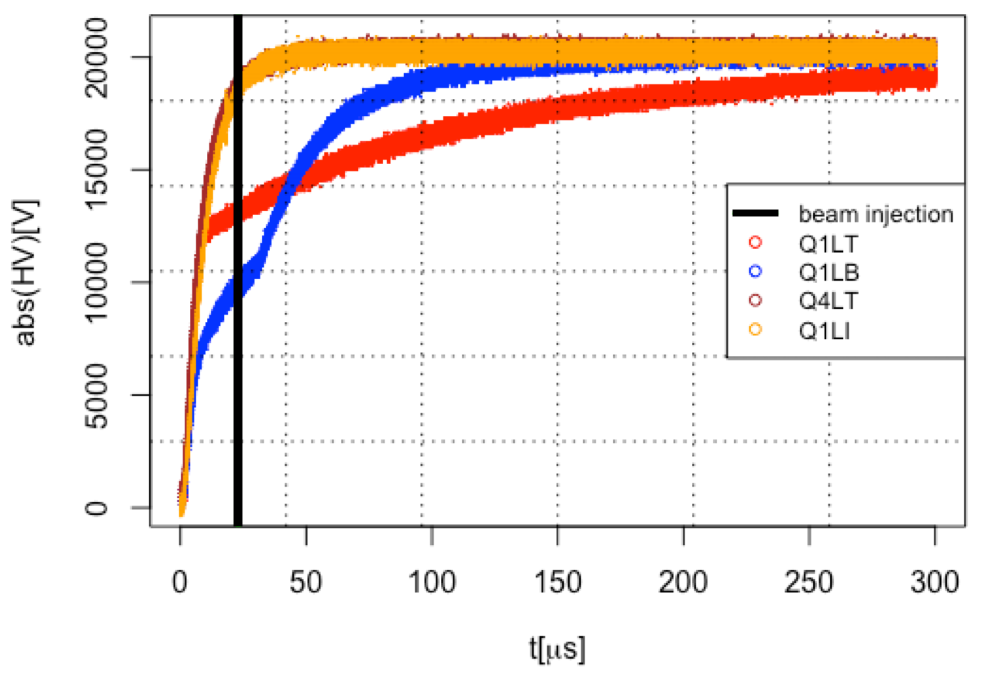
\includegraphics[width=.8\textwidth]{QuadTraces}
    \caption[Electrostatic quadrupole high voltage traces]{Traces for some quadrupole plate potentials as a function of time. The different plates are identified in the legend, where for instance Q1LT stands for the top long plate of quadrupole 1. The muon beam is injected into the ring at the black line and the scraping procedure occurs until the quadrupole voltages reach their design values, in this case $\SI{20.4}{kV}$. As shown some of the high voltage traces do not behave in a smooth and fast exponential manner, due to damaged quadrupole resistors. The traces in orange and brown are for good quadrupole resistors, while the traces in red and blue show the results from damaged quadrupole resistors. The kink in blue is the switch from the scraping procedure to storage.}
    \label{fig:QuadTraces}
\end{figure}


All data listed in \tabref{tab:Run1Datasets} were quality checked. If run conditions were found to be unsatisfactory, the associated data was flagged and ignored in the analysis. A summary of the data quality control procedure is given in \refref{DQCSummary}, and the exact data quality parameters for the 60h dataset are detailed in \refref{DQC60H}. The total number of detected positrons above threshold that passed the data quality control was approximately $\SI{1e10}{}$, corresponding to a statistical error on \wa of $\sim\SI{400}{ppb}$, as calculated with \equref{eq:waprecision}.




